\documentclass[twoside]{book}

% Packages required by doxygen
\usepackage{fixltx2e}
\usepackage{calc}
\usepackage{doxygen}
\usepackage[export]{adjustbox} % also loads graphicx
\usepackage{graphicx}
\usepackage[utf8]{inputenc}
\usepackage{makeidx}
\usepackage{multicol}
\usepackage{multirow}
\PassOptionsToPackage{warn}{textcomp}
\usepackage{textcomp}
\usepackage[nointegrals]{wasysym}
\usepackage[table]{xcolor}

% Font selection
\usepackage[T1]{fontenc}
\usepackage[scaled=.90]{helvet}
\usepackage{courier}
\usepackage{amssymb}
\usepackage{sectsty}
\renewcommand{\familydefault}{\sfdefault}
\allsectionsfont{%
  \fontseries{bc}\selectfont%
  \color{darkgray}%
}
\renewcommand{\DoxyLabelFont}{%
  \fontseries{bc}\selectfont%
  \color{darkgray}%
}
\newcommand{\+}{\discretionary{\mbox{\scriptsize$\hookleftarrow$}}{}{}}

% Page & text layout
\usepackage{geometry}
\geometry{%
  a4paper,%
  top=2.5cm,%
  bottom=2.5cm,%
  left=2.5cm,%
  right=2.5cm%
}
\tolerance=750
\hfuzz=15pt
\hbadness=750
\setlength{\emergencystretch}{15pt}
\setlength{\parindent}{0cm}
\setlength{\parskip}{3ex plus 2ex minus 2ex}
\makeatletter
\renewcommand{\paragraph}{%
  \@startsection{paragraph}{4}{0ex}{-1.0ex}{1.0ex}{%
    \normalfont\normalsize\bfseries\SS@parafont%
  }%
}
\renewcommand{\subparagraph}{%
  \@startsection{subparagraph}{5}{0ex}{-1.0ex}{1.0ex}{%
    \normalfont\normalsize\bfseries\SS@subparafont%
  }%
}
\makeatother

% Headers & footers
\usepackage{fancyhdr}
\pagestyle{fancyplain}
\fancyhead[LE]{\fancyplain{}{\bfseries\thepage}}
\fancyhead[CE]{\fancyplain{}{}}
\fancyhead[RE]{\fancyplain{}{\bfseries\leftmark}}
\fancyhead[LO]{\fancyplain{}{\bfseries\rightmark}}
\fancyhead[CO]{\fancyplain{}{}}
\fancyhead[RO]{\fancyplain{}{\bfseries\thepage}}
\fancyfoot[LE]{\fancyplain{}{}}
\fancyfoot[CE]{\fancyplain{}{}}
\fancyfoot[RE]{\fancyplain{}{\bfseries\scriptsize Generated by Doxygen }}
\fancyfoot[LO]{\fancyplain{}{\bfseries\scriptsize Generated by Doxygen }}
\fancyfoot[CO]{\fancyplain{}{}}
\fancyfoot[RO]{\fancyplain{}{}}
\renewcommand{\footrulewidth}{0.4pt}
\renewcommand{\chaptermark}[1]{%
  \markboth{#1}{}%
}
\renewcommand{\sectionmark}[1]{%
  \markright{\thesection\ #1}%
}

% Indices & bibliography
\usepackage{natbib}
\usepackage[titles]{tocloft}
\setcounter{tocdepth}{3}
\setcounter{secnumdepth}{5}
\makeindex

% Hyperlinks (required, but should be loaded last)
\usepackage{ifpdf}
\ifpdf
  \usepackage[pdftex,pagebackref=true]{hyperref}
\else
  \usepackage[ps2pdf,pagebackref=true]{hyperref}
\fi
\hypersetup{%
  colorlinks=true,%
  linkcolor=blue,%
  citecolor=blue,%
  unicode%
}

% Custom commands
\newcommand{\clearemptydoublepage}{%
  \newpage{\pagestyle{empty}\cleardoublepage}%
}

\usepackage{caption}
\captionsetup{labelsep=space,justification=centering,font={bf},singlelinecheck=off,skip=4pt,position=top}

%===== C O N T E N T S =====

\begin{document}

% Titlepage & ToC
\hypersetup{pageanchor=false,
             bookmarksnumbered=true,
             pdfencoding=unicode
            }
\pagenumbering{roman}
\begin{titlepage}
\vspace*{7cm}
\begin{center}%
{\Large G\+A\+ME }\\
\vspace*{1cm}
{\large Generated by Doxygen 1.8.11}\\
\end{center}
\end{titlepage}
\clearemptydoublepage
\tableofcontents
\clearemptydoublepage
\pagenumbering{arabic}
\hypersetup{pageanchor=true}

%--- Begin generated contents ---
\chapter{Class Index}
\section{Data Structures}
Here are the data structures with brief descriptions\+:\begin{DoxyCompactList}
\item\contentsline{section}{\hyperlink{structbackground}{background} }{\pageref{structbackground}}{}
\item\contentsline{section}{\hyperlink{structennemi}{ennemi} }{\pageref{structennemi}}{}
\item\contentsline{section}{\hyperlink{structpersonnage}{personnage} }{\pageref{structpersonnage}}{}
\item\contentsline{section}{\hyperlink{structscore}{score} }{\pageref{structscore}}{}
\item\contentsline{section}{\hyperlink{structtimer}{timer} }{\pageref{structtimer}}{}
\item\contentsline{section}{\hyperlink{structvie}{vie} }{\pageref{structvie}}{}
\end{DoxyCompactList}

\chapter{File Index}
\section{File List}
Here is a list of all files with brief descriptions\+:\begin{DoxyCompactList}
\item\contentsline{section}{\hyperlink{main_8c}{main.\+c} }{\pageref{main_8c}}{}
\item\contentsline{section}{\hyperlink{perso_8c}{perso.\+c} }{\pageref{perso_8c}}{}
\item\contentsline{section}{\hyperlink{perso_8h}{perso.\+h} }{\pageref{perso_8h}}{}
\end{DoxyCompactList}

\chapter{Class Documentation}
\hypertarget{structbackground}{}\section{background Struct Reference}
\label{structbackground}\index{background@{background}}


struct for background  




{\ttfamily \#include $<$save.\+h$>$}

\subsection*{Public Attributes}
\begin{DoxyCompactItemize}
\item 
S\+D\+L\+\_\+\+Surface $\ast$ \hyperlink{structbackground_a1c5c3a3ebb56924b9f829602f9641006}{img}
\item 
S\+D\+L\+\_\+\+Rect \hyperlink{structbackground_aa70f1467505f43c50fec228c21bd7af4}{pos}
\end{DoxyCompactItemize}


\subsection{Detailed Description}
struct for background 

\subsection{Member Data Documentation}
\index{background@{background}!img@{img}}
\index{img@{img}!background@{background}}
\subsubsection[{\texorpdfstring{img}{img}}]{\setlength{\rightskip}{0pt plus 5cm}S\+D\+L\+\_\+\+Surface$\ast$ background\+::img}\hypertarget{structbackground_a1c5c3a3ebb56924b9f829602f9641006}{}\label{structbackground_a1c5c3a3ebb56924b9f829602f9641006}
\index{background@{background}!pos@{pos}}
\index{pos@{pos}!background@{background}}
\subsubsection[{\texorpdfstring{pos}{pos}}]{\setlength{\rightskip}{0pt plus 5cm}S\+D\+L\+\_\+\+Rect background\+::pos}\hypertarget{structbackground_aa70f1467505f43c50fec228c21bd7af4}{}\label{structbackground_aa70f1467505f43c50fec228c21bd7af4}


The documentation for this struct was generated from the following file\+:\begin{DoxyCompactItemize}
\item 
\hyperlink{save_8h}{save.\+h}\end{DoxyCompactItemize}

\hypertarget{structennemi}{}\section{ennemi Struct Reference}
\label{structennemi}\index{ennemi@{ennemi}}


{\ttfamily \#include $<$save.\+h$>$}

\subsection*{Public Attributes}
\begin{DoxyCompactItemize}
\item 
S\+D\+L\+\_\+\+Rect \hyperlink{structennemi_ab236808a3af75588847442504250d02f}{position\+\_\+ennemi}
\item 
S\+D\+L\+\_\+\+Rect \hyperlink{structennemi_a1fca83eeee08fde8a80a8b9c0a0ae00f}{pos2}
\item 
S\+D\+L\+\_\+\+Rect \hyperlink{structennemi_a04c7d21c26dd2fd99eceecd6059bff90}{pos1}
\item 
S\+D\+L\+\_\+\+Rect \hyperlink{structennemi_abc473e1ffbf2e5848151d900724e3f83}{position\+\_\+sprite}
\item 
int \hyperlink{structennemi_aa1f57a616910ffd5799f1097a3160e0b}{direction}
\item 
S\+D\+L\+\_\+\+Surface $\ast$ \hyperlink{structennemi_a4f333ffffb5036c74a62a60437d60422}{spriteleft}
\item 
S\+D\+L\+\_\+\+Surface $\ast$ \hyperlink{structennemi_a8ad9de831604958b2654c033280129f1}{spriteright}
\end{DoxyCompactItemize}


\subsection{Member Data Documentation}
\index{ennemi@{ennemi}!direction@{direction}}
\index{direction@{direction}!ennemi@{ennemi}}
\subsubsection[{\texorpdfstring{direction}{direction}}]{\setlength{\rightskip}{0pt plus 5cm}int ennemi\+::direction}\hypertarget{structennemi_aa1f57a616910ffd5799f1097a3160e0b}{}\label{structennemi_aa1f57a616910ffd5799f1097a3160e0b}
\index{ennemi@{ennemi}!pos1@{pos1}}
\index{pos1@{pos1}!ennemi@{ennemi}}
\subsubsection[{\texorpdfstring{pos1}{pos1}}]{\setlength{\rightskip}{0pt plus 5cm}S\+D\+L\+\_\+\+Rect ennemi\+::pos1}\hypertarget{structennemi_a04c7d21c26dd2fd99eceecd6059bff90}{}\label{structennemi_a04c7d21c26dd2fd99eceecd6059bff90}
\index{ennemi@{ennemi}!pos2@{pos2}}
\index{pos2@{pos2}!ennemi@{ennemi}}
\subsubsection[{\texorpdfstring{pos2}{pos2}}]{\setlength{\rightskip}{0pt plus 5cm}S\+D\+L\+\_\+\+Rect ennemi\+::pos2}\hypertarget{structennemi_a1fca83eeee08fde8a80a8b9c0a0ae00f}{}\label{structennemi_a1fca83eeee08fde8a80a8b9c0a0ae00f}
\index{ennemi@{ennemi}!position\+\_\+ennemi@{position\+\_\+ennemi}}
\index{position\+\_\+ennemi@{position\+\_\+ennemi}!ennemi@{ennemi}}
\subsubsection[{\texorpdfstring{position\+\_\+ennemi}{position_ennemi}}]{\setlength{\rightskip}{0pt plus 5cm}S\+D\+L\+\_\+\+Rect ennemi\+::position\+\_\+ennemi}\hypertarget{structennemi_ab236808a3af75588847442504250d02f}{}\label{structennemi_ab236808a3af75588847442504250d02f}
\index{ennemi@{ennemi}!position\+\_\+sprite@{position\+\_\+sprite}}
\index{position\+\_\+sprite@{position\+\_\+sprite}!ennemi@{ennemi}}
\subsubsection[{\texorpdfstring{position\+\_\+sprite}{position_sprite}}]{\setlength{\rightskip}{0pt plus 5cm}S\+D\+L\+\_\+\+Rect ennemi\+::position\+\_\+sprite}\hypertarget{structennemi_abc473e1ffbf2e5848151d900724e3f83}{}\label{structennemi_abc473e1ffbf2e5848151d900724e3f83}
\index{ennemi@{ennemi}!spriteleft@{spriteleft}}
\index{spriteleft@{spriteleft}!ennemi@{ennemi}}
\subsubsection[{\texorpdfstring{spriteleft}{spriteleft}}]{\setlength{\rightskip}{0pt plus 5cm}S\+D\+L\+\_\+\+Surface$\ast$ ennemi\+::spriteleft}\hypertarget{structennemi_a4f333ffffb5036c74a62a60437d60422}{}\label{structennemi_a4f333ffffb5036c74a62a60437d60422}
\index{ennemi@{ennemi}!spriteright@{spriteright}}
\index{spriteright@{spriteright}!ennemi@{ennemi}}
\subsubsection[{\texorpdfstring{spriteright}{spriteright}}]{\setlength{\rightskip}{0pt plus 5cm}S\+D\+L\+\_\+\+Surface$\ast$ ennemi\+::spriteright}\hypertarget{structennemi_a8ad9de831604958b2654c033280129f1}{}\label{structennemi_a8ad9de831604958b2654c033280129f1}


The documentation for this struct was generated from the following file\+:\begin{DoxyCompactItemize}
\item 
\hyperlink{save_8h}{save.\+h}\end{DoxyCompactItemize}

\hypertarget{structObjet}{}\section{Objet Struct Reference}
\label{structObjet}\index{Objet@{Objet}}


{\ttfamily \#include $<$save.\+h$>$}

\subsection*{Public Attributes}
\begin{DoxyCompactItemize}
\item 
S\+D\+L\+\_\+\+Surface $\ast$ \hyperlink{structObjet_a0dac95199f82a456854968bfe257a14e}{img}
\item 
S\+D\+L\+\_\+\+Rect \hyperlink{structObjet_aa96c8e462a0637c98ab3c192e7f1806a}{pos}
\item 
S\+D\+L\+\_\+\+Rect \hyperlink{structObjet_a22b5f8635c29778f8a669585ec6ed6fd}{pos\+\_\+text}
\end{DoxyCompactItemize}


\subsection{Member Data Documentation}
\index{Objet@{Objet}!img@{img}}
\index{img@{img}!Objet@{Objet}}
\subsubsection[{\texorpdfstring{img}{img}}]{\setlength{\rightskip}{0pt plus 5cm}S\+D\+L\+\_\+\+Surface$\ast$ Objet\+::img}\hypertarget{structObjet_a0dac95199f82a456854968bfe257a14e}{}\label{structObjet_a0dac95199f82a456854968bfe257a14e}
\index{Objet@{Objet}!pos@{pos}}
\index{pos@{pos}!Objet@{Objet}}
\subsubsection[{\texorpdfstring{pos}{pos}}]{\setlength{\rightskip}{0pt plus 5cm}S\+D\+L\+\_\+\+Rect Objet\+::pos}\hypertarget{structObjet_aa96c8e462a0637c98ab3c192e7f1806a}{}\label{structObjet_aa96c8e462a0637c98ab3c192e7f1806a}
\index{Objet@{Objet}!pos\+\_\+text@{pos\+\_\+text}}
\index{pos\+\_\+text@{pos\+\_\+text}!Objet@{Objet}}
\subsubsection[{\texorpdfstring{pos\+\_\+text}{pos_text}}]{\setlength{\rightskip}{0pt plus 5cm}S\+D\+L\+\_\+\+Rect Objet\+::pos\+\_\+text}\hypertarget{structObjet_a22b5f8635c29778f8a669585ec6ed6fd}{}\label{structObjet_a22b5f8635c29778f8a669585ec6ed6fd}


The documentation for this struct was generated from the following file\+:\begin{DoxyCompactItemize}
\item 
\hyperlink{save_8h}{save.\+h}\end{DoxyCompactItemize}

\hypertarget{structobjet}{}\section{objet Struct Reference}
\label{structobjet}\index{objet@{objet}}


struct for yes/no objet  




{\ttfamily \#include $<$save.\+h$>$}



\subsection{Detailed Description}
struct for yes/no objet 

The documentation for this struct was generated from the following file\+:\begin{DoxyCompactItemize}
\item 
\hyperlink{save_8h}{save.\+h}\end{DoxyCompactItemize}

\hypertarget{structpersonnage}{}\section{personnage Struct Reference}
\label{structpersonnage}\index{personnage@{personnage}}


{\ttfamily \#include $<$struct.\+h$>$}



Collaboration diagram for personnage\+:
\nopagebreak
\begin{figure}[H]
\begin{center}
\leavevmode
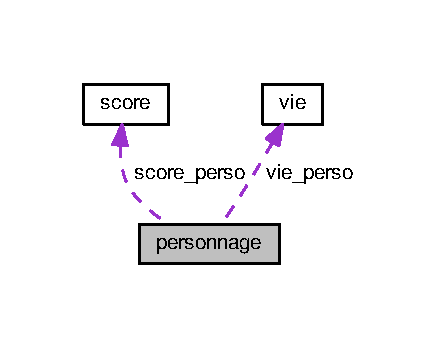
\includegraphics[width=211pt]{structpersonnage__coll__graph}
\end{center}
\end{figure}
\subsection*{Data Fields}
\begin{DoxyCompactItemize}
\item 
S\+D\+L\+\_\+\+Surface $\ast$ \hyperlink{structpersonnage_a3fc8b5a6848cc4b09b844f482411a414}{sprite} \mbox{[}12\mbox{]}
\item 
S\+D\+L\+\_\+\+Rect \hyperlink{structpersonnage_a4a45c9e4310d819fcd3c9a60fc8c0ebf}{position\+\_\+perso}
\item 
int \hyperlink{structpersonnage_a2664acffa6fccd8487b9e03b63fbd6da}{direction}
\item 
\hyperlink{structvie}{vie} \hyperlink{structpersonnage_ac96f4aee44111bc31a7718e5762bf483}{vie\+\_\+perso}
\item 
\hyperlink{structscore}{score} \hyperlink{structpersonnage_a7ea99b7d0c8445cb3d7ba6717eb89d8c}{score\+\_\+perso}
\item 
int \hyperlink{structpersonnage_acfac32928075716cc10265cfc9f551fc}{num}
\end{DoxyCompactItemize}


\subsection{Field Documentation}
\mbox{\Hypertarget{structpersonnage_a2664acffa6fccd8487b9e03b63fbd6da}\label{structpersonnage_a2664acffa6fccd8487b9e03b63fbd6da}} 
\index{personnage@{personnage}!direction@{direction}}
\index{direction@{direction}!personnage@{personnage}}
\subsubsection{\texorpdfstring{direction}{direction}}
{\footnotesize\ttfamily int personnage\+::direction}

\mbox{\Hypertarget{structpersonnage_acfac32928075716cc10265cfc9f551fc}\label{structpersonnage_acfac32928075716cc10265cfc9f551fc}} 
\index{personnage@{personnage}!num@{num}}
\index{num@{num}!personnage@{personnage}}
\subsubsection{\texorpdfstring{num}{num}}
{\footnotesize\ttfamily int personnage\+::num}

\mbox{\Hypertarget{structpersonnage_a4a45c9e4310d819fcd3c9a60fc8c0ebf}\label{structpersonnage_a4a45c9e4310d819fcd3c9a60fc8c0ebf}} 
\index{personnage@{personnage}!position\+\_\+perso@{position\+\_\+perso}}
\index{position\+\_\+perso@{position\+\_\+perso}!personnage@{personnage}}
\subsubsection{\texorpdfstring{position\+\_\+perso}{position\_perso}}
{\footnotesize\ttfamily S\+D\+L\+\_\+\+Rect personnage\+::position\+\_\+perso}

\mbox{\Hypertarget{structpersonnage_a7ea99b7d0c8445cb3d7ba6717eb89d8c}\label{structpersonnage_a7ea99b7d0c8445cb3d7ba6717eb89d8c}} 
\index{personnage@{personnage}!score\+\_\+perso@{score\+\_\+perso}}
\index{score\+\_\+perso@{score\+\_\+perso}!personnage@{personnage}}
\subsubsection{\texorpdfstring{score\+\_\+perso}{score\_perso}}
{\footnotesize\ttfamily \hyperlink{structscore}{score} personnage\+::score\+\_\+perso}

\mbox{\Hypertarget{structpersonnage_a3fc8b5a6848cc4b09b844f482411a414}\label{structpersonnage_a3fc8b5a6848cc4b09b844f482411a414}} 
\index{personnage@{personnage}!sprite@{sprite}}
\index{sprite@{sprite}!personnage@{personnage}}
\subsubsection{\texorpdfstring{sprite}{sprite}}
{\footnotesize\ttfamily S\+D\+L\+\_\+\+Surface$\ast$ personnage\+::sprite\mbox{[}12\mbox{]}}

\mbox{\Hypertarget{structpersonnage_ac96f4aee44111bc31a7718e5762bf483}\label{structpersonnage_ac96f4aee44111bc31a7718e5762bf483}} 
\index{personnage@{personnage}!vie\+\_\+perso@{vie\+\_\+perso}}
\index{vie\+\_\+perso@{vie\+\_\+perso}!personnage@{personnage}}
\subsubsection{\texorpdfstring{vie\+\_\+perso}{vie\_perso}}
{\footnotesize\ttfamily \hyperlink{structvie}{vie} personnage\+::vie\+\_\+perso}



The documentation for this struct was generated from the following file\+:\begin{DoxyCompactItemize}
\item 
\hyperlink{struct_8h}{struct.\+h}\end{DoxyCompactItemize}

\hypertarget{structscore}{}\section{score Struct Reference}
\label{structscore}\index{score@{score}}


struct for score of hero  




{\ttfamily \#include $<$perso.\+h$>$}

\subsection*{Public Attributes}
\begin{DoxyCompactItemize}
\item 
int \hyperlink{structscore_a86ee1f22a5bf4e92781f2b2165aa0859}{score\+\_\+atteint}
\item 
S\+D\+L\+\_\+\+Rect \hyperlink{structscore_a444e826e64d1abf14dc0108095752cc1}{position\+\_\+score}
\item 
T\+T\+F\+\_\+\+Font $\ast$ \hyperlink{structscore_aa8088c00f0a0ce91db39deb03afc7110}{police\+\_\+score}
\item 
S\+D\+L\+\_\+\+Surface $\ast$ \hyperlink{structscore_aa5918332d1797da4bedaccfce5446b88}{score\+\_\+texte}
\end{DoxyCompactItemize}


\subsection{Detailed Description}
struct for score of hero 

\subsection{Member Data Documentation}
\index{score@{score}!police\+\_\+score@{police\+\_\+score}}
\index{police\+\_\+score@{police\+\_\+score}!score@{score}}
\subsubsection[{\texorpdfstring{police\+\_\+score}{police_score}}]{\setlength{\rightskip}{0pt plus 5cm}T\+T\+F\+\_\+\+Font$\ast$ score\+::police\+\_\+score}\hypertarget{structscore_aa8088c00f0a0ce91db39deb03afc7110}{}\label{structscore_aa8088c00f0a0ce91db39deb03afc7110}
font \index{score@{score}!position\+\_\+score@{position\+\_\+score}}
\index{position\+\_\+score@{position\+\_\+score}!score@{score}}
\subsubsection[{\texorpdfstring{position\+\_\+score}{position_score}}]{\setlength{\rightskip}{0pt plus 5cm}S\+D\+L\+\_\+\+Rect score\+::position\+\_\+score}\hypertarget{structscore_a444e826e64d1abf14dc0108095752cc1}{}\label{structscore_a444e826e64d1abf14dc0108095752cc1}
rectangle \index{score@{score}!score\+\_\+atteint@{score\+\_\+atteint}}
\index{score\+\_\+atteint@{score\+\_\+atteint}!score@{score}}
\subsubsection[{\texorpdfstring{score\+\_\+atteint}{score_atteint}}]{\setlength{\rightskip}{0pt plus 5cm}int score\+::score\+\_\+atteint}\hypertarget{structscore_a86ee1f22a5bf4e92781f2b2165aa0859}{}\label{structscore_a86ee1f22a5bf4e92781f2b2165aa0859}
entier \index{score@{score}!score\+\_\+texte@{score\+\_\+texte}}
\index{score\+\_\+texte@{score\+\_\+texte}!score@{score}}
\subsubsection[{\texorpdfstring{score\+\_\+texte}{score_texte}}]{\setlength{\rightskip}{0pt plus 5cm}S\+D\+L\+\_\+\+Surface$\ast$ score\+::score\+\_\+texte}\hypertarget{structscore_aa5918332d1797da4bedaccfce5446b88}{}\label{structscore_aa5918332d1797da4bedaccfce5446b88}
surface 

The documentation for this struct was generated from the following file\+:\begin{DoxyCompactItemize}
\item 
\hyperlink{perso_8h}{perso.\+h}\end{DoxyCompactItemize}

\hypertarget{structvie}{}\section{vie Struct Reference}
\label{structvie}\index{vie@{vie}}


struct for vie perso  




{\ttfamily \#include $<$save.\+h$>$}

\subsection*{Public Attributes}
\begin{DoxyCompactItemize}
\item 
int \hyperlink{structvie_ace0f84a19ce4f5854ec56c137b33b947}{nbredevie}
\item 
S\+D\+L\+\_\+\+Surface $\ast$ \hyperlink{structvie_a2c29f60898de16e1306bd1043fa38dc9}{vie} \mbox{[}4\mbox{]}
\item 
S\+D\+L\+\_\+\+Rect \hyperlink{structvie_aaa37f269f7261984f2e540534210af5a}{position\+\_\+de\+\_\+vie}
\end{DoxyCompactItemize}


\subsection{Detailed Description}
struct for vie perso 

\subsection{Member Data Documentation}
\index{vie@{vie}!nbredevie@{nbredevie}}
\index{nbredevie@{nbredevie}!vie@{vie}}
\subsubsection[{\texorpdfstring{nbredevie}{nbredevie}}]{\setlength{\rightskip}{0pt plus 5cm}int vie\+::nbredevie}\hypertarget{structvie_ace0f84a19ce4f5854ec56c137b33b947}{}\label{structvie_ace0f84a19ce4f5854ec56c137b33b947}
entier \index{vie@{vie}!position\+\_\+de\+\_\+vie@{position\+\_\+de\+\_\+vie}}
\index{position\+\_\+de\+\_\+vie@{position\+\_\+de\+\_\+vie}!vie@{vie}}
\subsubsection[{\texorpdfstring{position\+\_\+de\+\_\+vie}{position_de_vie}}]{\setlength{\rightskip}{0pt plus 5cm}S\+D\+L\+\_\+\+Rect vie\+::position\+\_\+de\+\_\+vie}\hypertarget{structvie_aaa37f269f7261984f2e540534210af5a}{}\label{structvie_aaa37f269f7261984f2e540534210af5a}
rectangle \index{vie@{vie}!vie@{vie}}
\index{vie@{vie}!vie@{vie}}
\subsubsection[{\texorpdfstring{vie}{vie}}]{\setlength{\rightskip}{0pt plus 5cm}S\+D\+L\+\_\+\+Surface$\ast$ vie\+::vie\mbox{[}4\mbox{]}}\hypertarget{structvie_a2c29f60898de16e1306bd1043fa38dc9}{}\label{structvie_a2c29f60898de16e1306bd1043fa38dc9}
surface 

The documentation for this struct was generated from the following file\+:\begin{DoxyCompactItemize}
\item 
\hyperlink{save_8h}{save.\+h}\end{DoxyCompactItemize}

\chapter{File Documentation}
\hypertarget{mainsave_8c}{}\section{mainsave.\+c File Reference}
\label{mainsave_8c}\index{mainsave.\+c@{mainsave.\+c}}
{\ttfamily \#include \char`\"{}save.\+h\char`\"{}}\\*
{\ttfamily \#include $<$stdio.\+h$>$}\\*
{\ttfamily \#include $<$stdlib.\+h$>$}\\*
{\ttfamily \#include $<$math.\+h$>$}\\*
{\ttfamily \#include \char`\"{}S\+D\+L/\+S\+D\+L.\+h\char`\"{}}\\*
{\ttfamily \#include \char`\"{}S\+D\+L/\+S\+D\+L\+\_\+image.\+h\char`\"{}}\\*
{\ttfamily \#include \char`\"{}S\+D\+L/\+S\+D\+L\+\_\+mixer.\+h\char`\"{}}\\*
{\ttfamily \#include \char`\"{}S\+D\+L/\+S\+D\+L\+\_\+ttf.\+h\char`\"{}}\\*
Include dependency graph for mainsave.\+c\+:\nopagebreak
\begin{figure}[H]
\begin{center}
\leavevmode
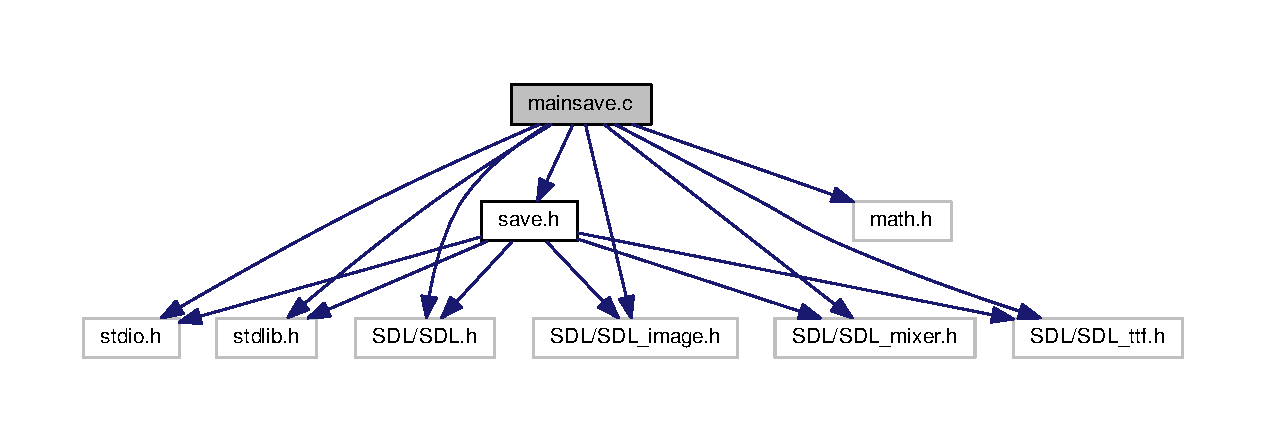
\includegraphics[width=350pt]{mainsave_8c__incl}
\end{center}
\end{figure}
\subsection*{Functions}
\begin{DoxyCompactItemize}
\item 
int \hyperlink{mainsave_8c_ae66f6b31b5ad750f1fe042a706a4e3d4}{main} ()
\end{DoxyCompactItemize}


\subsection{Detailed Description}
Bouabker Arij \begin{DoxyDate}{Date}
Mai ,2020
\end{DoxyDate}
testing program for game saving and loading 

\subsection{Function Documentation}
\index{mainsave.\+c@{mainsave.\+c}!main@{main}}
\index{main@{main}!mainsave.\+c@{mainsave.\+c}}
\subsubsection[{\texorpdfstring{main()}{main()}}]{\setlength{\rightskip}{0pt plus 5cm}int main (
\begin{DoxyParamCaption}
{}
\end{DoxyParamCaption}
)}\hypertarget{mainsave_8c_ae66f6b31b5ad750f1fe042a706a4e3d4}{}\label{mainsave_8c_ae66f6b31b5ad750f1fe042a706a4e3d4}


Here is the call graph for this function\+:
\nopagebreak
\begin{figure}[H]
\begin{center}
\leavevmode
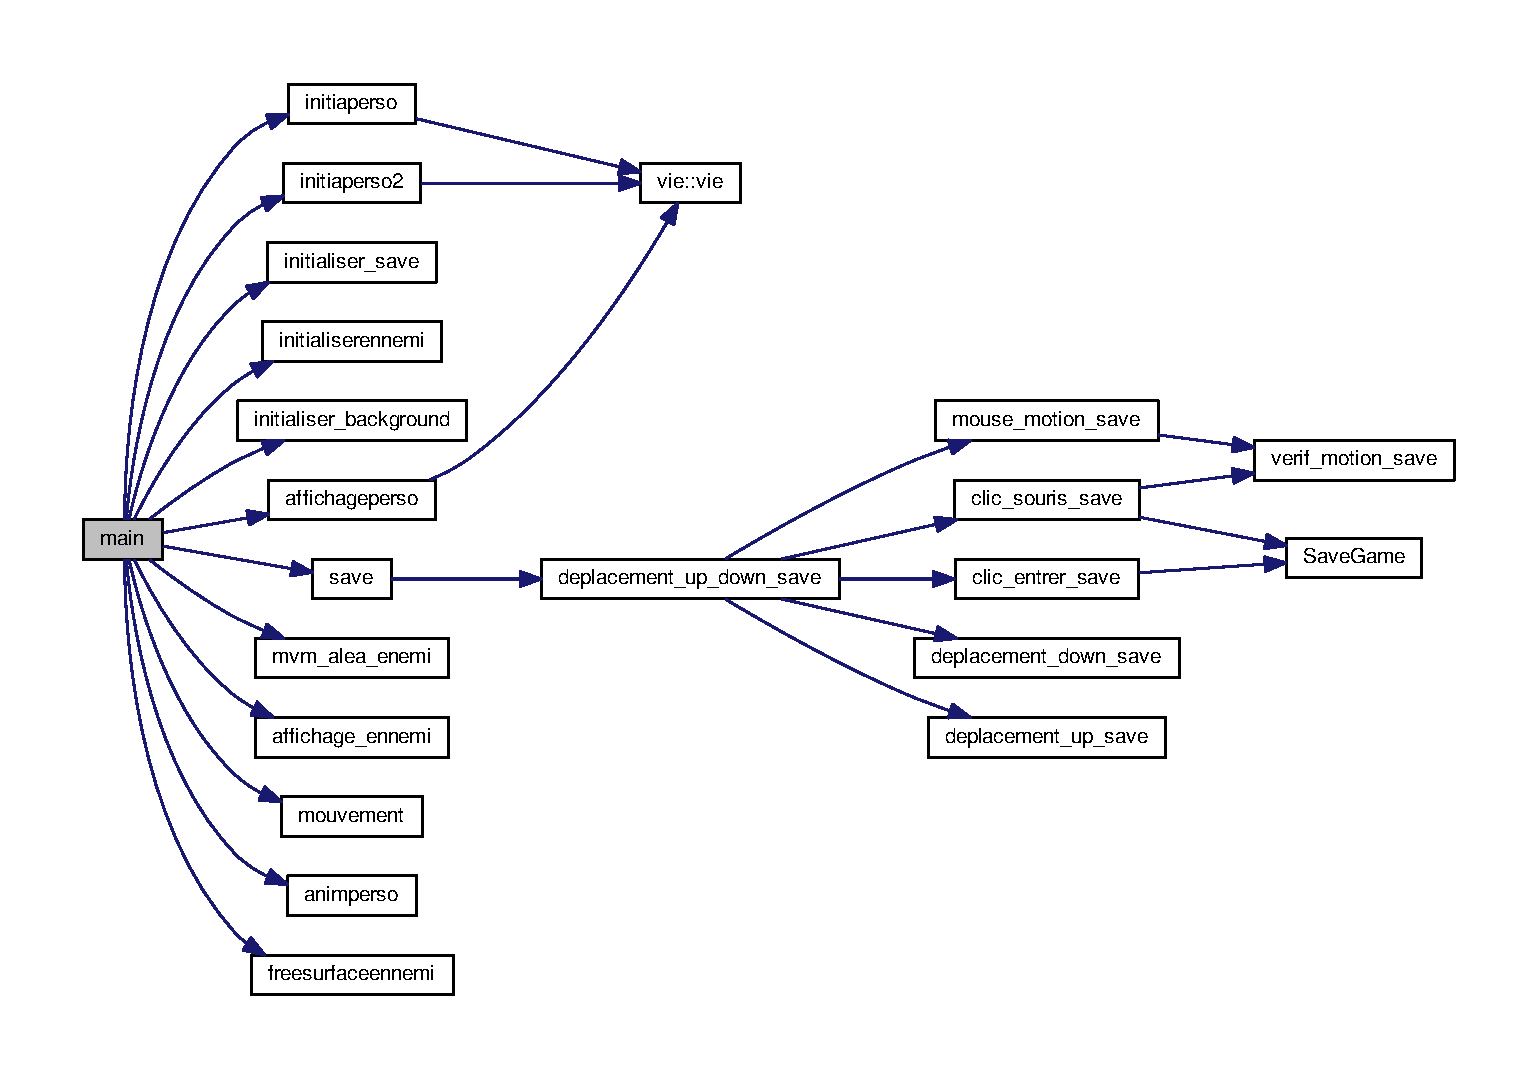
\includegraphics[width=350pt]{mainsave_8c_ae66f6b31b5ad750f1fe042a706a4e3d4_cgraph}
\end{center}
\end{figure}



\hypertarget{save_8c}{}\section{save.\+c File Reference}
\label{save_8c}\index{save.\+c@{save.\+c}}
{\ttfamily \#include \char`\"{}save.\+h\char`\"{}}\\*
{\ttfamily \#include $<$stdio.\+h$>$}\\*
{\ttfamily \#include $<$stdlib.\+h$>$}\\*
{\ttfamily \#include $<$math.\+h$>$}\\*
{\ttfamily \#include \char`\"{}S\+D\+L/\+S\+D\+L.\+h\char`\"{}}\\*
{\ttfamily \#include \char`\"{}S\+D\+L/\+S\+D\+L\+\_\+image.\+h\char`\"{}}\\*
{\ttfamily \#include \char`\"{}S\+D\+L/\+S\+D\+L\+\_\+mixer.\+h\char`\"{}}\\*
{\ttfamily \#include \char`\"{}S\+D\+L/\+S\+D\+L\+\_\+ttf.\+h\char`\"{}}\\*
Include dependency graph for save.\+c\+:\nopagebreak
\begin{figure}[H]
\begin{center}
\leavevmode
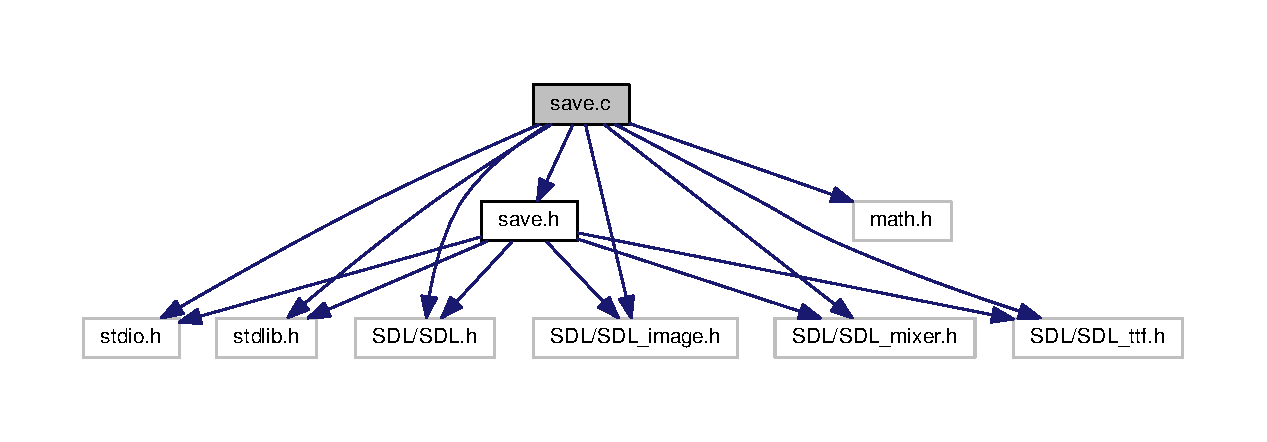
\includegraphics[width=350pt]{save_8c__incl}
\end{center}
\end{figure}
\subsection*{Functions}
\begin{DoxyCompactItemize}
\item 
\hyperlink{structpersonnage}{personnage} \hyperlink{save_8c_a8fd5cd633f844d0f565c513d966ecc2a}{initperso} (\hyperlink{structpersonnage}{personnage} c, int posx, int posy, int posw, int posh, int direction, int posviex, int posviey, int nbre\+\_\+de\+\_\+vie, int \hyperlink{structscore}{score}, int spritex, int spritey, int spritew, int spriteh, int numr, int numl, int posscorex, int posscorey, int velocity, int speed, int i)
\begin{DoxyCompactList}\small\item\em to initialize hero \end{DoxyCompactList}\item 
\hyperlink{structbackground}{background} \hyperlink{save_8c_a99dd96b8f84fbb251e26afc643890b8a}{initialiser\+\_\+background} (\hyperlink{structbackground}{background} b, int posx, int posy, int i)
\begin{DoxyCompactList}\small\item\em to initialize background \end{DoxyCompactList}\item 
\hyperlink{structennemi}{ennemi} \hyperlink{save_8c_a1237b088a523ece0f6f69491c5252e2e}{initialiser\+\_\+ennemi} (\hyperlink{structennemi}{ennemi} e, int eposition\+\_\+ennemix, int eposition\+\_\+ennemiy, int epos1x, int epos1y, int epos2x, int epos2y, int eposition\+\_\+spritex, int eposition\+\_\+spritey, int eposition\+\_\+spritew, int eposition\+\_\+spriteh, int edirection)
\begin{DoxyCompactList}\small\item\em to initialize ennemy \end{DoxyCompactList}\item 
void \hyperlink{save_8c_a936a0790f87300c4d50a1fe7959875f5}{mouvement} (\hyperlink{structpersonnage}{personnage} $\ast$c)
\begin{DoxyCompactList}\small\item\em to move hero \end{DoxyCompactList}\item 
void \hyperlink{save_8c_a37690785871acb57ed11799088bec266}{animperso} (\hyperlink{structpersonnage}{personnage} $\ast$c, S\+D\+L\+\_\+\+Surface $\ast$screen)
\begin{DoxyCompactList}\small\item\em to animate hero \end{DoxyCompactList}\item 
void \hyperlink{save_8c_a4fcd9448740c67449649edb846515fae}{affichageperso} (\hyperlink{structpersonnage}{personnage} c, S\+D\+L\+\_\+\+Surface $\ast$screen)
\begin{DoxyCompactList}\small\item\em to display hero \end{DoxyCompactList}\item 
void \hyperlink{save_8c_a30a06a7282f7de8937717af0b47b31cb}{Save\+Game} (\hyperlink{structpersonnage}{personnage} c1, \hyperlink{structpersonnage}{personnage} c2, \hyperlink{structbackground}{background} b, char $\ast$file, \hyperlink{structennemi}{ennemi} e, int niveau)
\begin{DoxyCompactList}\small\item\em to save game \end{DoxyCompactList}\item 
void \hyperlink{save_8c_acb4f6e609d2abc8783d41104e804ebf6}{initialiser\+\_\+save} (\hyperlink{structObjet}{Objet} $\ast$sauv, \hyperlink{structObjet}{Objet} $\ast$sauvy, \hyperlink{structObjet}{Objet} $\ast$sauvn)
\begin{DoxyCompactList}\small\item\em pour initialiser le menu de save oui/non \end{DoxyCompactList}\item 
int \hyperlink{save_8c_a323063e0b0a6c01cd3f01617e0df1d6e}{verif\+\_\+motion\+\_\+save} (S\+D\+L\+\_\+\+Event event, \hyperlink{structObjet}{Objet} surface)
\begin{DoxyCompactList}\small\item\em to verify mouse motion \end{DoxyCompactList}\item 
void \hyperlink{save_8c_a6897cc2439ee8a56c0d55f5e17bcd4dc}{clic\+\_\+souris\+\_\+save} (S\+D\+L\+\_\+\+Surface $\ast$screen, S\+D\+L\+\_\+\+Event event, int curseur, \hyperlink{structObjet}{Objet} sauvn, \hyperlink{structObjet}{Objet} sauvy, \hyperlink{structpersonnage}{personnage} c1, \hyperlink{structpersonnage}{personnage} c2, \hyperlink{structbackground}{background} b, char $\ast$file, \hyperlink{structennemi}{ennemi} e, int niveau)
\begin{DoxyCompactList}\small\item\em clic avec souris dans le menu de save oui/non \end{DoxyCompactList}\item 
void \hyperlink{save_8c_acd785e84ec9a4180b7686e73da03dd26}{clic\+\_\+entrer\+\_\+save} (S\+D\+L\+\_\+\+Surface $\ast$screen, Mix\+\_\+\+Chunk $\ast$effect, int curseur, \hyperlink{structObjet}{Objet} sauvn, \hyperlink{structObjet}{Objet} sauvy, \hyperlink{structpersonnage}{personnage} c1, \hyperlink{structpersonnage}{personnage} c2, \hyperlink{structbackground}{background} b, char $\ast$file, \hyperlink{structennemi}{ennemi} e, int niveau)
\begin{DoxyCompactList}\small\item\em clic avec bouton entrer dans le menu de save oui/non \end{DoxyCompactList}\item 
void \hyperlink{save_8c_a26ae7b755f8291e47249e059641a1cb5}{mouse\+\_\+motion\+\_\+save} (S\+D\+L\+\_\+\+Surface $\ast$screen, S\+D\+L\+\_\+\+Event event, Mix\+\_\+\+Chunk $\ast$effect, int $\ast$curseur, \hyperlink{structObjet}{Objet} sauvn, \hyperlink{structObjet}{Objet} sauvy)
\begin{DoxyCompactList}\small\item\em mouse motion dans le menu de save oui/non \end{DoxyCompactList}\item 
void \hyperlink{save_8c_a7fcb6ded09f67d099c5ec72e874d2261}{deplacement\+\_\+down\+\_\+save} (S\+D\+L\+\_\+\+Surface $\ast$screen, Mix\+\_\+\+Chunk $\ast$effect, int $\ast$curseur, \hyperlink{structObjet}{Objet} sauvn, \hyperlink{structObjet}{Objet} sauvy)
\begin{DoxyCompactList}\small\item\em se deplacer vers le bas dans le menu de save oui/non \end{DoxyCompactList}\item 
void \hyperlink{save_8c_a3d9d3c3144b808484894caf3bdded4fe}{deplacement\+\_\+up\+\_\+save} (S\+D\+L\+\_\+\+Surface $\ast$screen, Mix\+\_\+\+Chunk $\ast$effect, int $\ast$curseur, \hyperlink{structObjet}{Objet} sauvn, \hyperlink{structObjet}{Objet} sauvy)
\begin{DoxyCompactList}\small\item\em se deplacer vers le haut dans le menu de save oui/non \end{DoxyCompactList}\item 
int \hyperlink{save_8c_ae98bea39bce363158739b999ebc38ceb}{deplacement\+\_\+up\+\_\+down\+\_\+save} (S\+D\+L\+\_\+\+Surface $\ast$screen, S\+D\+L\+\_\+\+Event event, int $\ast$curseur, \hyperlink{structObjet}{Objet} sauvn, \hyperlink{structObjet}{Objet} sauvy, Mix\+\_\+\+Chunk $\ast$effect, int $\ast$go, \hyperlink{structpersonnage}{personnage} c1, \hyperlink{structpersonnage}{personnage} c2, \hyperlink{structbackground}{background} b, char $\ast$file, \hyperlink{structennemi}{ennemi} e, int niveau)
\begin{DoxyCompactList}\small\item\em se deplacer vers le bas et vers le haut dans le menu de save oui/non \end{DoxyCompactList}\item 
int \hyperlink{save_8c_a34e892752d1de82a8306307f2e7dbfb7}{save} (S\+D\+L\+\_\+\+Surface $\ast$screen, S\+D\+L\+\_\+\+Event event, int $\ast$curseur, \hyperlink{structObjet}{Objet} sauv, \hyperlink{structObjet}{Objet} sauvn, \hyperlink{structObjet}{Objet} sauvy, Mix\+\_\+\+Chunk $\ast$effect, \hyperlink{structpersonnage}{personnage} c1, \hyperlink{structpersonnage}{personnage} c2, \hyperlink{structbackground}{background} b, char $\ast$file, \hyperlink{structennemi}{ennemi} e, int niveau, int $\ast$go)
\begin{DoxyCompactList}\small\item\em to save game \end{DoxyCompactList}\item 
void \hyperlink{save_8c_a18376703725eb8a89b00df24948bee5f}{Load\+Game} (\hyperlink{structpersonnage}{personnage} $\ast$c1, \hyperlink{structpersonnage}{personnage} $\ast$c2, \hyperlink{structbackground}{background} $\ast$b, \hyperlink{structennemi}{ennemi} $\ast$e, int $\ast$niveau, S\+D\+L\+\_\+\+Surface $\ast$screen)
\begin{DoxyCompactList}\small\item\em to load game \end{DoxyCompactList}\item 
void \hyperlink{save_8c_ad429715f94be9c05e0f873efd01f62ff}{freesurfaceennemi} (\hyperlink{structennemi}{ennemi} $\ast$e)
\begin{DoxyCompactList}\small\item\em 

 \end{DoxyCompactList}\item 
void \hyperlink{save_8c_ad7f4f5d982725341ae87b93b9b1a91fc}{affichage\+\_\+ennemi} (\hyperlink{structennemi}{ennemi} e, S\+D\+L\+\_\+\+Surface $\ast$screen)
\begin{DoxyCompactList}\small\item\em 

 \end{DoxyCompactList}\item 
void \hyperlink{save_8c_a5b88fedc1de2481522fa32569e5b7393}{mvm\+\_\+alea\+\_\+enemi} (\hyperlink{structennemi}{ennemi} $\ast$e)
\begin{DoxyCompactList}\small\item\em 

 \end{DoxyCompactList}\item 
void \hyperlink{save_8c_a449db8c266f1c795e8de1e9e9802f90b}{initialiserennemi} (\hyperlink{structennemi}{ennemi} $\ast$e)
\begin{DoxyCompactList}\small\item\em to initialize ennemy \end{DoxyCompactList}\item 
\hyperlink{structpersonnage}{personnage} \hyperlink{save_8c_ad6b94a0d07757d441340deb27a5d26fe}{initiaperso} (\hyperlink{structpersonnage}{personnage} c)
\item 
\hyperlink{structpersonnage}{personnage} \hyperlink{save_8c_abc15402f1bc9be9a242db8d4f9403b4e}{initiaperso2} (\hyperlink{structpersonnage}{personnage} c)
\end{DoxyCompactItemize}


\subsection{Detailed Description}
Bouabker Arij \begin{DoxyDate}{Date}
Mai ,2020
\end{DoxyDate}
testing program for game saving anad loading 

\subsection{Function Documentation}
\index{save.\+c@{save.\+c}!affichage\+\_\+ennemi@{affichage\+\_\+ennemi}}
\index{affichage\+\_\+ennemi@{affichage\+\_\+ennemi}!save.\+c@{save.\+c}}
\subsubsection[{\texorpdfstring{affichage\+\_\+ennemi(ennemi e, S\+D\+L\+\_\+\+Surface $\ast$screen)}{affichage_ennemi(ennemi e, SDL_Surface *screen)}}]{\setlength{\rightskip}{0pt plus 5cm}void affichage\+\_\+ennemi (
\begin{DoxyParamCaption}
\item[{{\bf ennemi}}]{e, }
\item[{S\+D\+L\+\_\+\+Surface $\ast$}]{screen}
\end{DoxyParamCaption}
)}\hypertarget{save_8c_ad7f4f5d982725341ae87b93b9b1a91fc}{}\label{save_8c_ad7f4f5d982725341ae87b93b9b1a91fc}




 

to display ennemy 
\begin{DoxyParams}{Parameters}
{\em screen} & \\
\hline
{\em e=ennemi} & \\
\hline
\end{DoxyParams}
\begin{DoxyReturn}{Returns}
nothing 
\end{DoxyReturn}


Here is the caller graph for this function\+:\nopagebreak
\begin{figure}[H]
\begin{center}
\leavevmode
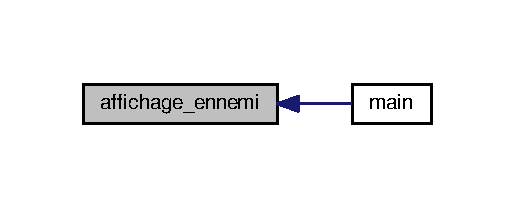
\includegraphics[width=247pt]{save_8c_ad7f4f5d982725341ae87b93b9b1a91fc_icgraph}
\end{center}
\end{figure}


\index{save.\+c@{save.\+c}!affichageperso@{affichageperso}}
\index{affichageperso@{affichageperso}!save.\+c@{save.\+c}}
\subsubsection[{\texorpdfstring{affichageperso(personnage c, S\+D\+L\+\_\+\+Surface $\ast$screen)}{affichageperso(personnage c, SDL_Surface *screen)}}]{\setlength{\rightskip}{0pt plus 5cm}void affichageperso (
\begin{DoxyParamCaption}
\item[{{\bf personnage}}]{c, }
\item[{S\+D\+L\+\_\+\+Surface $\ast$}]{screen}
\end{DoxyParamCaption}
)}\hypertarget{save_8c_a4fcd9448740c67449649edb846515fae}{}\label{save_8c_a4fcd9448740c67449649edb846515fae}


to display hero 


\begin{DoxyParams}{Parameters}
{\em c=personnage} & \\
\hline
{\em screen} & \\
\hline
\end{DoxyParams}
\begin{DoxyReturn}{Returns}
nothing 
\end{DoxyReturn}


Here is the call graph for this function\+:\nopagebreak
\begin{figure}[H]
\begin{center}
\leavevmode
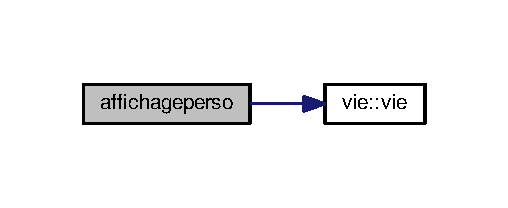
\includegraphics[width=244pt]{save_8c_a4fcd9448740c67449649edb846515fae_cgraph}
\end{center}
\end{figure}




Here is the caller graph for this function\+:\nopagebreak
\begin{figure}[H]
\begin{center}
\leavevmode
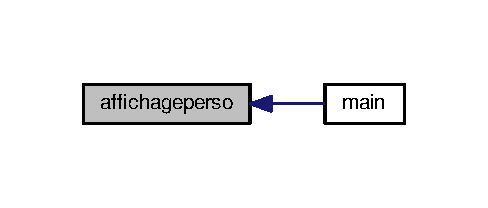
\includegraphics[width=234pt]{save_8c_a4fcd9448740c67449649edb846515fae_icgraph}
\end{center}
\end{figure}


\index{save.\+c@{save.\+c}!animperso@{animperso}}
\index{animperso@{animperso}!save.\+c@{save.\+c}}
\subsubsection[{\texorpdfstring{animperso(personnage $\ast$c, S\+D\+L\+\_\+\+Surface $\ast$screen)}{animperso(personnage *c, SDL_Surface *screen)}}]{\setlength{\rightskip}{0pt plus 5cm}void animperso (
\begin{DoxyParamCaption}
\item[{{\bf personnage} $\ast$}]{c, }
\item[{S\+D\+L\+\_\+\+Surface $\ast$}]{screen}
\end{DoxyParamCaption}
)}\hypertarget{save_8c_a37690785871acb57ed11799088bec266}{}\label{save_8c_a37690785871acb57ed11799088bec266}


to animate hero 


\begin{DoxyParams}{Parameters}
{\em c=personnage} & \\
\hline
{\em screen} & \\
\hline
\end{DoxyParams}
\begin{DoxyReturn}{Returns}
nothing 
\end{DoxyReturn}


Here is the caller graph for this function\+:\nopagebreak
\begin{figure}[H]
\begin{center}
\leavevmode
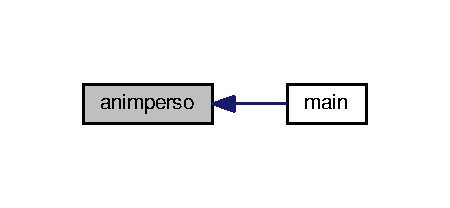
\includegraphics[width=216pt]{save_8c_a37690785871acb57ed11799088bec266_icgraph}
\end{center}
\end{figure}


\index{save.\+c@{save.\+c}!clic\+\_\+entrer\+\_\+save@{clic\+\_\+entrer\+\_\+save}}
\index{clic\+\_\+entrer\+\_\+save@{clic\+\_\+entrer\+\_\+save}!save.\+c@{save.\+c}}
\subsubsection[{\texorpdfstring{clic\+\_\+entrer\+\_\+save(\+S\+D\+L\+\_\+\+Surface $\ast$screen, Mix\+\_\+\+Chunk $\ast$effect, int curseur, Objet sauvn, Objet sauvy, personnage c1, personnage c2, background b, char $\ast$file, ennemi e, int niveau)}{clic_entrer_save(SDL_Surface *screen, Mix_Chunk *effect, int curseur, Objet sauvn, Objet sauvy, personnage c1, personnage c2, background b, char *file, ennemi e, int niveau)}}]{\setlength{\rightskip}{0pt plus 5cm}void clic\+\_\+entrer\+\_\+save (
\begin{DoxyParamCaption}
\item[{S\+D\+L\+\_\+\+Surface $\ast$}]{screen, }
\item[{Mix\+\_\+\+Chunk $\ast$}]{effect, }
\item[{int}]{curseur, }
\item[{{\bf Objet}}]{sauvn, }
\item[{{\bf Objet}}]{sauvy, }
\item[{{\bf personnage}}]{c1, }
\item[{{\bf personnage}}]{c2, }
\item[{{\bf background}}]{b, }
\item[{char $\ast$}]{file, }
\item[{{\bf ennemi}}]{e, }
\item[{int}]{niveau}
\end{DoxyParamCaption}
)}\hypertarget{save_8c_acd785e84ec9a4180b7686e73da03dd26}{}\label{save_8c_acd785e84ec9a4180b7686e73da03dd26}


clic avec bouton entrer dans le menu de save oui/non 


\begin{DoxyParams}{Parameters}
{\em screen} & \\
\hline
{\em effect} & \\
\hline
{\em curseur} & \\
\hline
{\em sauvy} & \\
\hline
{\em sauvn} & \\
\hline
{\em c1=personnage} & 1 \\
\hline
{\em c2=personnage} & 2 \\
\hline
{\em b=background} & \\
\hline
{\em file} & \\
\hline
{\em e=ennemy} & \\
\hline
{\em niveau} & \\
\hline
\end{DoxyParams}
\begin{DoxyReturn}{Returns}
nothing 
\end{DoxyReturn}


Here is the call graph for this function\+:\nopagebreak
\begin{figure}[H]
\begin{center}
\leavevmode
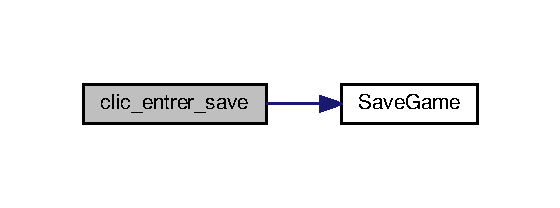
\includegraphics[width=269pt]{save_8c_acd785e84ec9a4180b7686e73da03dd26_cgraph}
\end{center}
\end{figure}




Here is the caller graph for this function\+:
\nopagebreak
\begin{figure}[H]
\begin{center}
\leavevmode
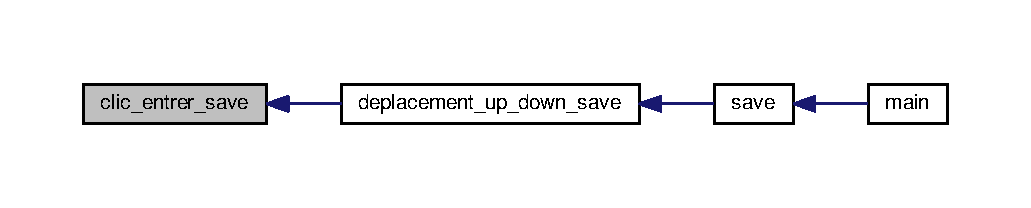
\includegraphics[width=350pt]{save_8c_acd785e84ec9a4180b7686e73da03dd26_icgraph}
\end{center}
\end{figure}


\index{save.\+c@{save.\+c}!clic\+\_\+souris\+\_\+save@{clic\+\_\+souris\+\_\+save}}
\index{clic\+\_\+souris\+\_\+save@{clic\+\_\+souris\+\_\+save}!save.\+c@{save.\+c}}
\subsubsection[{\texorpdfstring{clic\+\_\+souris\+\_\+save(\+S\+D\+L\+\_\+\+Surface $\ast$screen, S\+D\+L\+\_\+\+Event event, int curseur, Objet sauvn, Objet sauvy, personnage c1, personnage c2, background b, char $\ast$file, ennemi e, int niveau)}{clic_souris_save(SDL_Surface *screen, SDL_Event event, int curseur, Objet sauvn, Objet sauvy, personnage c1, personnage c2, background b, char *file, ennemi e, int niveau)}}]{\setlength{\rightskip}{0pt plus 5cm}void clic\+\_\+souris\+\_\+save (
\begin{DoxyParamCaption}
\item[{S\+D\+L\+\_\+\+Surface $\ast$}]{screen, }
\item[{S\+D\+L\+\_\+\+Event}]{event, }
\item[{int}]{curseur, }
\item[{{\bf Objet}}]{sauvn, }
\item[{{\bf Objet}}]{sauvy, }
\item[{{\bf personnage}}]{c1, }
\item[{{\bf personnage}}]{c2, }
\item[{{\bf background}}]{b, }
\item[{char $\ast$}]{file, }
\item[{{\bf ennemi}}]{e, }
\item[{int}]{niveau}
\end{DoxyParamCaption}
)}\hypertarget{save_8c_a6897cc2439ee8a56c0d55f5e17bcd4dc}{}\label{save_8c_a6897cc2439ee8a56c0d55f5e17bcd4dc}


clic avec souris dans le menu de save oui/non 


\begin{DoxyParams}{Parameters}
{\em screen} & \\
\hline
{\em event} & \\
\hline
{\em curseur} & \\
\hline
{\em sauvy} & \\
\hline
{\em sauvn} & \\
\hline
{\em c1=personnage} & 1 \\
\hline
{\em c2=personnage} & 2 \\
\hline
{\em b=background} & \\
\hline
{\em file} & \\
\hline
{\em e=ennemy} & \\
\hline
{\em niveau} & \\
\hline
\end{DoxyParams}
\begin{DoxyReturn}{Returns}
nothing 
\end{DoxyReturn}


Here is the call graph for this function\+:\nopagebreak
\begin{figure}[H]
\begin{center}
\leavevmode
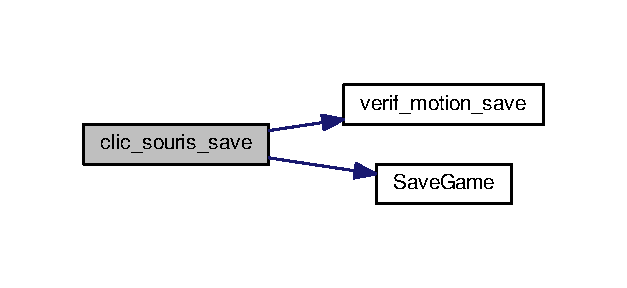
\includegraphics[width=301pt]{save_8c_a6897cc2439ee8a56c0d55f5e17bcd4dc_cgraph}
\end{center}
\end{figure}




Here is the caller graph for this function\+:
\nopagebreak
\begin{figure}[H]
\begin{center}
\leavevmode
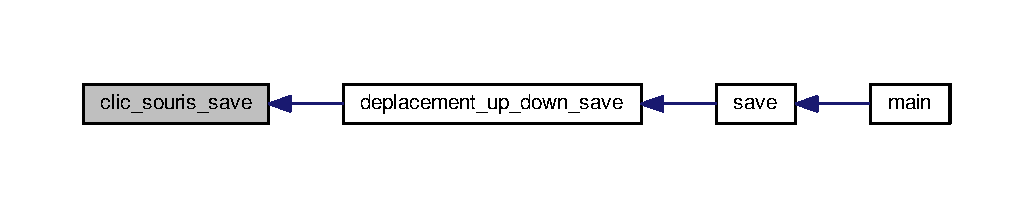
\includegraphics[width=350pt]{save_8c_a6897cc2439ee8a56c0d55f5e17bcd4dc_icgraph}
\end{center}
\end{figure}


\index{save.\+c@{save.\+c}!deplacement\+\_\+down\+\_\+save@{deplacement\+\_\+down\+\_\+save}}
\index{deplacement\+\_\+down\+\_\+save@{deplacement\+\_\+down\+\_\+save}!save.\+c@{save.\+c}}
\subsubsection[{\texorpdfstring{deplacement\+\_\+down\+\_\+save(\+S\+D\+L\+\_\+\+Surface $\ast$screen, Mix\+\_\+\+Chunk $\ast$effect, int $\ast$curseur, Objet sauvn, Objet sauvy)}{deplacement_down_save(SDL_Surface *screen, Mix_Chunk *effect, int *curseur, Objet sauvn, Objet sauvy)}}]{\setlength{\rightskip}{0pt plus 5cm}void deplacement\+\_\+down\+\_\+save (
\begin{DoxyParamCaption}
\item[{S\+D\+L\+\_\+\+Surface $\ast$}]{screen, }
\item[{Mix\+\_\+\+Chunk $\ast$}]{effect, }
\item[{int $\ast$}]{curseur, }
\item[{{\bf Objet}}]{sauvn, }
\item[{{\bf Objet}}]{sauvy}
\end{DoxyParamCaption}
)}\hypertarget{save_8c_a7fcb6ded09f67d099c5ec72e874d2261}{}\label{save_8c_a7fcb6ded09f67d099c5ec72e874d2261}


se deplacer vers le bas dans le menu de save oui/non 


\begin{DoxyParams}{Parameters}
{\em screen} & \\
\hline
{\em sauvn} & \\
\hline
{\em sauvy} & \\
\hline
{\em curseur} & \\
\hline
{\em effect} & \\
\hline
\end{DoxyParams}
\begin{DoxyReturn}{Returns}
nothing 
\end{DoxyReturn}


Here is the caller graph for this function\+:
\nopagebreak
\begin{figure}[H]
\begin{center}
\leavevmode
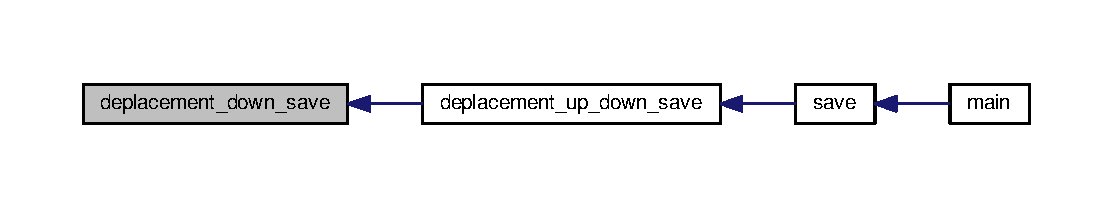
\includegraphics[width=350pt]{save_8c_a7fcb6ded09f67d099c5ec72e874d2261_icgraph}
\end{center}
\end{figure}


\index{save.\+c@{save.\+c}!deplacement\+\_\+up\+\_\+down\+\_\+save@{deplacement\+\_\+up\+\_\+down\+\_\+save}}
\index{deplacement\+\_\+up\+\_\+down\+\_\+save@{deplacement\+\_\+up\+\_\+down\+\_\+save}!save.\+c@{save.\+c}}
\subsubsection[{\texorpdfstring{deplacement\+\_\+up\+\_\+down\+\_\+save(\+S\+D\+L\+\_\+\+Surface $\ast$screen, S\+D\+L\+\_\+\+Event event, int $\ast$curseur, Objet sauvn, Objet sauvy, Mix\+\_\+\+Chunk $\ast$effect, int $\ast$go, personnage c1, personnage c2, background b, char $\ast$file, ennemi e, int niveau)}{deplacement_up_down_save(SDL_Surface *screen, SDL_Event event, int *curseur, Objet sauvn, Objet sauvy, Mix_Chunk *effect, int *go, personnage c1, personnage c2, background b, char *file, ennemi e, int niveau)}}]{\setlength{\rightskip}{0pt plus 5cm}int deplacement\+\_\+up\+\_\+down\+\_\+save (
\begin{DoxyParamCaption}
\item[{S\+D\+L\+\_\+\+Surface $\ast$}]{screen, }
\item[{S\+D\+L\+\_\+\+Event}]{event, }
\item[{int $\ast$}]{curseur, }
\item[{{\bf Objet}}]{sauvn, }
\item[{{\bf Objet}}]{sauvy, }
\item[{Mix\+\_\+\+Chunk $\ast$}]{effect, }
\item[{int $\ast$}]{go, }
\item[{{\bf personnage}}]{c1, }
\item[{{\bf personnage}}]{c2, }
\item[{{\bf background}}]{b, }
\item[{char $\ast$}]{file, }
\item[{{\bf ennemi}}]{e, }
\item[{int}]{niveau}
\end{DoxyParamCaption}
)}\hypertarget{save_8c_ae98bea39bce363158739b999ebc38ceb}{}\label{save_8c_ae98bea39bce363158739b999ebc38ceb}


se deplacer vers le bas et vers le haut dans le menu de save oui/non 


\begin{DoxyParams}{Parameters}
{\em screen} & \\
\hline
{\em event} & \\
\hline
{\em curseur} & \\
\hline
{\em sauv} & \\
\hline
{\em sauvn} & \\
\hline
{\em sauvy} & \\
\hline
{\em effect} & \\
\hline
{\em c1=personnage} & 1 \\
\hline
{\em c2=personnage} & 2 \\
\hline
{\em b=background} & \\
\hline
{\em file} & \\
\hline
{\em e=ennemy} & \\
\hline
{\em niveau} & \\
\hline
{\em go} & \\
\hline
{\em c=personnage} & \\
\hline
\end{DoxyParams}
\begin{DoxyReturn}{Returns}
nothing 
\end{DoxyReturn}


Here is the call graph for this function\+:
\nopagebreak
\begin{figure}[H]
\begin{center}
\leavevmode
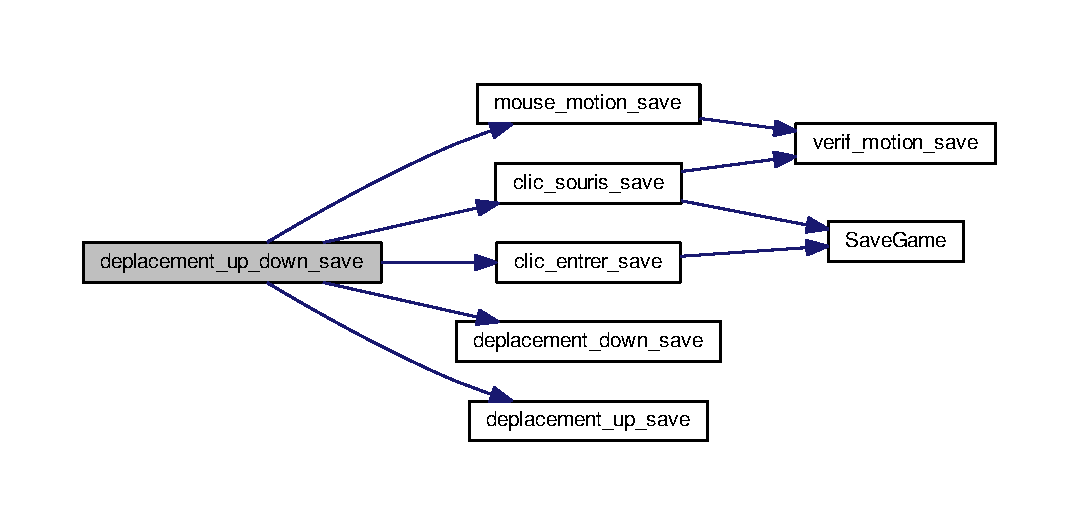
\includegraphics[width=350pt]{save_8c_ae98bea39bce363158739b999ebc38ceb_cgraph}
\end{center}
\end{figure}




Here is the caller graph for this function\+:
\nopagebreak
\begin{figure}[H]
\begin{center}
\leavevmode
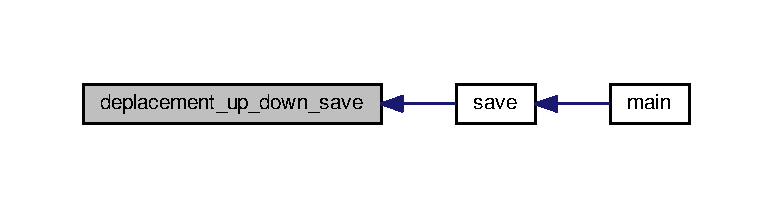
\includegraphics[width=350pt]{save_8c_ae98bea39bce363158739b999ebc38ceb_icgraph}
\end{center}
\end{figure}


\index{save.\+c@{save.\+c}!deplacement\+\_\+up\+\_\+save@{deplacement\+\_\+up\+\_\+save}}
\index{deplacement\+\_\+up\+\_\+save@{deplacement\+\_\+up\+\_\+save}!save.\+c@{save.\+c}}
\subsubsection[{\texorpdfstring{deplacement\+\_\+up\+\_\+save(\+S\+D\+L\+\_\+\+Surface $\ast$screen, Mix\+\_\+\+Chunk $\ast$effect, int $\ast$curseur, Objet sauvn, Objet sauvy)}{deplacement_up_save(SDL_Surface *screen, Mix_Chunk *effect, int *curseur, Objet sauvn, Objet sauvy)}}]{\setlength{\rightskip}{0pt plus 5cm}void deplacement\+\_\+up\+\_\+save (
\begin{DoxyParamCaption}
\item[{S\+D\+L\+\_\+\+Surface $\ast$}]{screen, }
\item[{Mix\+\_\+\+Chunk $\ast$}]{effect, }
\item[{int $\ast$}]{curseur, }
\item[{{\bf Objet}}]{sauvn, }
\item[{{\bf Objet}}]{sauvy}
\end{DoxyParamCaption}
)}\hypertarget{save_8c_a3d9d3c3144b808484894caf3bdded4fe}{}\label{save_8c_a3d9d3c3144b808484894caf3bdded4fe}


se deplacer vers le haut dans le menu de save oui/non 


\begin{DoxyParams}{Parameters}
{\em screen} & \\
\hline
{\em curseur} & \\
\hline
{\em sauvn} & \\
\hline
{\em sauvy} & \\
\hline
{\em effect} & \\
\hline
\end{DoxyParams}
\begin{DoxyReturn}{Returns}
nothing 
\end{DoxyReturn}


Here is the caller graph for this function\+:
\nopagebreak
\begin{figure}[H]
\begin{center}
\leavevmode
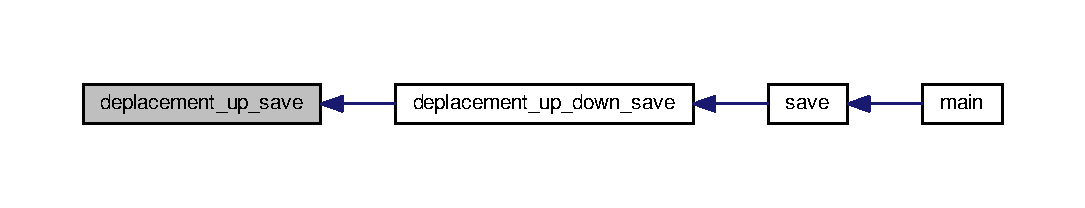
\includegraphics[width=350pt]{save_8c_a3d9d3c3144b808484894caf3bdded4fe_icgraph}
\end{center}
\end{figure}


\index{save.\+c@{save.\+c}!freesurfaceennemi@{freesurfaceennemi}}
\index{freesurfaceennemi@{freesurfaceennemi}!save.\+c@{save.\+c}}
\subsubsection[{\texorpdfstring{freesurfaceennemi(ennemi $\ast$e)}{freesurfaceennemi(ennemi *e)}}]{\setlength{\rightskip}{0pt plus 5cm}void freesurfaceennemi (
\begin{DoxyParamCaption}
\item[{{\bf ennemi} $\ast$}]{e}
\end{DoxyParamCaption}
)}\hypertarget{save_8c_ad429715f94be9c05e0f873efd01f62ff}{}\label{save_8c_ad429715f94be9c05e0f873efd01f62ff}




 

to free memory from ennemy 
\begin{DoxyParams}{Parameters}
{\em e=ennemi} & \\
\hline
\end{DoxyParams}
\begin{DoxyReturn}{Returns}
nothing 
\end{DoxyReturn}


Here is the caller graph for this function\+:\nopagebreak
\begin{figure}[H]
\begin{center}
\leavevmode
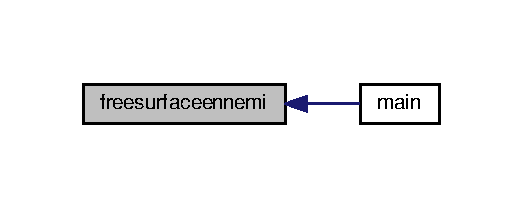
\includegraphics[width=251pt]{save_8c_ad429715f94be9c05e0f873efd01f62ff_icgraph}
\end{center}
\end{figure}


\index{save.\+c@{save.\+c}!initialiser\+\_\+background@{initialiser\+\_\+background}}
\index{initialiser\+\_\+background@{initialiser\+\_\+background}!save.\+c@{save.\+c}}
\subsubsection[{\texorpdfstring{initialiser\+\_\+background(background b, int posx, int posy, int i)}{initialiser_background(background b, int posx, int posy, int i)}}]{\setlength{\rightskip}{0pt plus 5cm}{\bf background} initialiser\+\_\+background (
\begin{DoxyParamCaption}
\item[{{\bf background}}]{b, }
\item[{int}]{posx, }
\item[{int}]{posy, }
\item[{int}]{i}
\end{DoxyParamCaption}
)}\hypertarget{save_8c_a99dd96b8f84fbb251e26afc643890b8a}{}\label{save_8c_a99dd96b8f84fbb251e26afc643890b8a}


to initialize background 

\begin{DoxyReturn}{Returns}
background 
\end{DoxyReturn}


Here is the caller graph for this function\+:\nopagebreak
\begin{figure}[H]
\begin{center}
\leavevmode
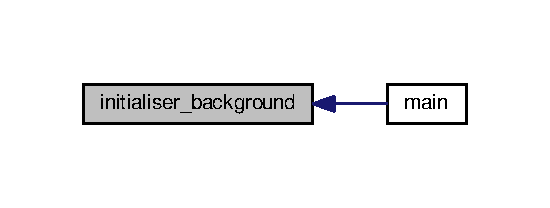
\includegraphics[width=264pt]{save_8c_a99dd96b8f84fbb251e26afc643890b8a_icgraph}
\end{center}
\end{figure}


\index{save.\+c@{save.\+c}!initialiser\+\_\+ennemi@{initialiser\+\_\+ennemi}}
\index{initialiser\+\_\+ennemi@{initialiser\+\_\+ennemi}!save.\+c@{save.\+c}}
\subsubsection[{\texorpdfstring{initialiser\+\_\+ennemi(ennemi e, int eposition\+\_\+ennemix, int eposition\+\_\+ennemiy, int epos1x, int epos1y, int epos2x, int epos2y, int eposition\+\_\+spritex, int eposition\+\_\+spritey, int eposition\+\_\+spritew, int eposition\+\_\+spriteh, int edirection)}{initialiser_ennemi(ennemi e, int eposition_ennemix, int eposition_ennemiy, int epos1x, int epos1y, int epos2x, int epos2y, int eposition_spritex, int eposition_spritey, int eposition_spritew, int eposition_spriteh, int edirection)}}]{\setlength{\rightskip}{0pt plus 5cm}{\bf ennemi} initialiser\+\_\+ennemi (
\begin{DoxyParamCaption}
\item[{{\bf ennemi}}]{e, }
\item[{int}]{eposition\+\_\+ennemix, }
\item[{int}]{eposition\+\_\+ennemiy, }
\item[{int}]{epos1x, }
\item[{int}]{epos1y, }
\item[{int}]{epos2x, }
\item[{int}]{epos2y, }
\item[{int}]{eposition\+\_\+spritex, }
\item[{int}]{eposition\+\_\+spritey, }
\item[{int}]{eposition\+\_\+spritew, }
\item[{int}]{eposition\+\_\+spriteh, }
\item[{int}]{edirection}
\end{DoxyParamCaption}
)}\hypertarget{save_8c_a1237b088a523ece0f6f69491c5252e2e}{}\label{save_8c_a1237b088a523ece0f6f69491c5252e2e}


to initialize ennemy 

\begin{DoxyReturn}{Returns}
ennemy 
\end{DoxyReturn}
\index{save.\+c@{save.\+c}!initialiser\+\_\+save@{initialiser\+\_\+save}}
\index{initialiser\+\_\+save@{initialiser\+\_\+save}!save.\+c@{save.\+c}}
\subsubsection[{\texorpdfstring{initialiser\+\_\+save(\+Objet $\ast$sauv, Objet $\ast$sauvy, Objet $\ast$sauvn)}{initialiser_save(Objet *sauv, Objet *sauvy, Objet *sauvn)}}]{\setlength{\rightskip}{0pt plus 5cm}void initialiser\+\_\+save (
\begin{DoxyParamCaption}
\item[{{\bf Objet} $\ast$}]{sauv, }
\item[{{\bf Objet} $\ast$}]{sauvy, }
\item[{{\bf Objet} $\ast$}]{sauvn}
\end{DoxyParamCaption}
)}\hypertarget{save_8c_acb4f6e609d2abc8783d41104e804ebf6}{}\label{save_8c_acb4f6e609d2abc8783d41104e804ebf6}


pour initialiser le menu de save oui/non 


\begin{DoxyParams}{Parameters}
{\em sauvy} & \\
\hline
{\em sauvn} & \\
\hline
{\em sauv} & \\
\hline
\end{DoxyParams}
\begin{DoxyReturn}{Returns}
nothing 
\end{DoxyReturn}


Here is the caller graph for this function\+:\nopagebreak
\begin{figure}[H]
\begin{center}
\leavevmode
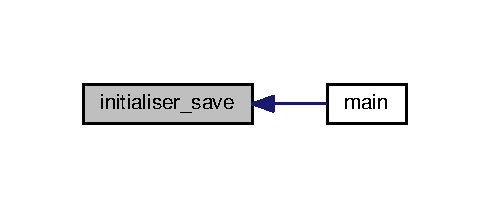
\includegraphics[width=235pt]{save_8c_acb4f6e609d2abc8783d41104e804ebf6_icgraph}
\end{center}
\end{figure}


\index{save.\+c@{save.\+c}!initialiserennemi@{initialiserennemi}}
\index{initialiserennemi@{initialiserennemi}!save.\+c@{save.\+c}}
\subsubsection[{\texorpdfstring{initialiserennemi(ennemi $\ast$e)}{initialiserennemi(ennemi *e)}}]{\setlength{\rightskip}{0pt plus 5cm}void initialiserennemi (
\begin{DoxyParamCaption}
\item[{{\bf ennemi} $\ast$}]{e}
\end{DoxyParamCaption}
)}\hypertarget{save_8c_a449db8c266f1c795e8de1e9e9802f90b}{}\label{save_8c_a449db8c266f1c795e8de1e9e9802f90b}


to initialize ennemy 





\begin{DoxyReturn}{Returns}
nothing 
\end{DoxyReturn}


Here is the caller graph for this function\+:\nopagebreak
\begin{figure}[H]
\begin{center}
\leavevmode
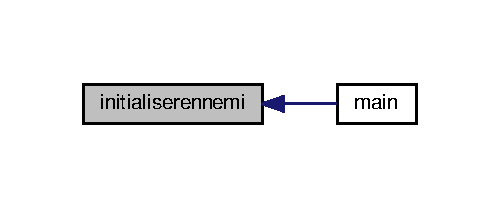
\includegraphics[width=240pt]{save_8c_a449db8c266f1c795e8de1e9e9802f90b_icgraph}
\end{center}
\end{figure}


\index{save.\+c@{save.\+c}!initiaperso@{initiaperso}}
\index{initiaperso@{initiaperso}!save.\+c@{save.\+c}}
\subsubsection[{\texorpdfstring{initiaperso(personnage c)}{initiaperso(personnage c)}}]{\setlength{\rightskip}{0pt plus 5cm}{\bf personnage} initiaperso (
\begin{DoxyParamCaption}
\item[{{\bf personnage}}]{c}
\end{DoxyParamCaption}
)}\hypertarget{save_8c_ad6b94a0d07757d441340deb27a5d26fe}{}\label{save_8c_ad6b94a0d07757d441340deb27a5d26fe}


Here is the call graph for this function\+:\nopagebreak
\begin{figure}[H]
\begin{center}
\leavevmode
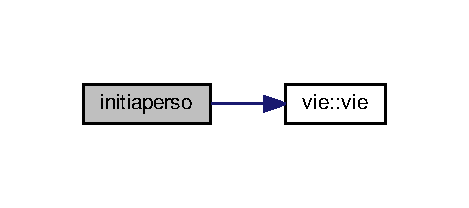
\includegraphics[width=225pt]{save_8c_ad6b94a0d07757d441340deb27a5d26fe_cgraph}
\end{center}
\end{figure}




Here is the caller graph for this function\+:\nopagebreak
\begin{figure}[H]
\begin{center}
\leavevmode
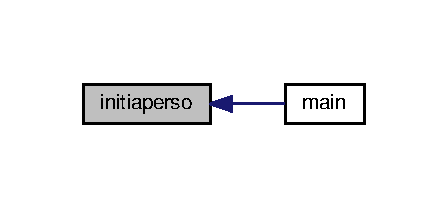
\includegraphics[width=215pt]{save_8c_ad6b94a0d07757d441340deb27a5d26fe_icgraph}
\end{center}
\end{figure}


\index{save.\+c@{save.\+c}!initiaperso2@{initiaperso2}}
\index{initiaperso2@{initiaperso2}!save.\+c@{save.\+c}}
\subsubsection[{\texorpdfstring{initiaperso2(personnage c)}{initiaperso2(personnage c)}}]{\setlength{\rightskip}{0pt plus 5cm}{\bf personnage} initiaperso2 (
\begin{DoxyParamCaption}
\item[{{\bf personnage}}]{c}
\end{DoxyParamCaption}
)}\hypertarget{save_8c_abc15402f1bc9be9a242db8d4f9403b4e}{}\label{save_8c_abc15402f1bc9be9a242db8d4f9403b4e}


Here is the call graph for this function\+:
\nopagebreak
\begin{figure}[H]
\begin{center}
\leavevmode
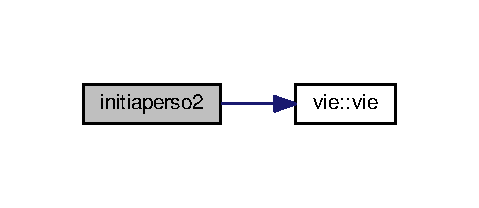
\includegraphics[width=230pt]{save_8c_abc15402f1bc9be9a242db8d4f9403b4e_cgraph}
\end{center}
\end{figure}




Here is the caller graph for this function\+:
\nopagebreak
\begin{figure}[H]
\begin{center}
\leavevmode
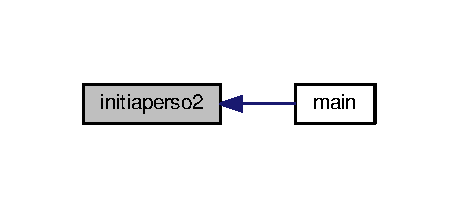
\includegraphics[width=220pt]{save_8c_abc15402f1bc9be9a242db8d4f9403b4e_icgraph}
\end{center}
\end{figure}


\index{save.\+c@{save.\+c}!initperso@{initperso}}
\index{initperso@{initperso}!save.\+c@{save.\+c}}
\subsubsection[{\texorpdfstring{initperso(personnage c, int posx, int posy, int posw, int posh, int direction, int posviex, int posviey, int nbre\+\_\+de\+\_\+vie, int score, int spritex, int spritey, int spritew, int spriteh, int numr, int numl, int posscorex, int posscorey, int velocity, int speed, int i)}{initperso(personnage c, int posx, int posy, int posw, int posh, int direction, int posviex, int posviey, int nbre_de_vie, int score, int spritex, int spritey, int spritew, int spriteh, int numr, int numl, int posscorex, int posscorey, int velocity, int speed, int i)}}]{\setlength{\rightskip}{0pt plus 5cm}{\bf personnage} initperso (
\begin{DoxyParamCaption}
\item[{{\bf personnage}}]{c, }
\item[{int}]{posx, }
\item[{int}]{posy, }
\item[{int}]{posw, }
\item[{int}]{posh, }
\item[{int}]{direction, }
\item[{int}]{posviex, }
\item[{int}]{posviey, }
\item[{int}]{nbre\+\_\+de\+\_\+vie, }
\item[{int}]{score, }
\item[{int}]{spritex, }
\item[{int}]{spritey, }
\item[{int}]{spritew, }
\item[{int}]{spriteh, }
\item[{int}]{numr, }
\item[{int}]{numl, }
\item[{int}]{posscorex, }
\item[{int}]{posscorey, }
\item[{int}]{velocity, }
\item[{int}]{speed, }
\item[{int}]{i}
\end{DoxyParamCaption}
)}\hypertarget{save_8c_a8fd5cd633f844d0f565c513d966ecc2a}{}\label{save_8c_a8fd5cd633f844d0f565c513d966ecc2a}


to initialize hero 

\begin{DoxyReturn}{Returns}
personnage 
\end{DoxyReturn}


Here is the call graph for this function\+:\nopagebreak
\begin{figure}[H]
\begin{center}
\leavevmode
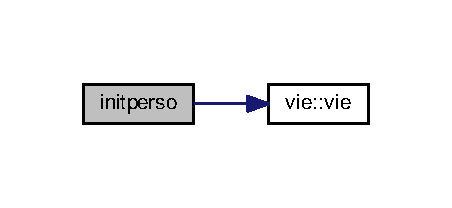
\includegraphics[width=217pt]{save_8c_a8fd5cd633f844d0f565c513d966ecc2a_cgraph}
\end{center}
\end{figure}


\index{save.\+c@{save.\+c}!Load\+Game@{Load\+Game}}
\index{Load\+Game@{Load\+Game}!save.\+c@{save.\+c}}
\subsubsection[{\texorpdfstring{Load\+Game(personnage $\ast$c1, personnage $\ast$c2, background $\ast$b, ennemi $\ast$e, int $\ast$niveau, S\+D\+L\+\_\+\+Surface $\ast$screen)}{LoadGame(personnage *c1, personnage *c2, background *b, ennemi *e, int *niveau, SDL_Surface *screen)}}]{\setlength{\rightskip}{0pt plus 5cm}void Load\+Game (
\begin{DoxyParamCaption}
\item[{{\bf personnage} $\ast$}]{c1, }
\item[{{\bf personnage} $\ast$}]{c2, }
\item[{{\bf background} $\ast$}]{b, }
\item[{{\bf ennemi} $\ast$}]{e, }
\item[{int $\ast$}]{niveau, }
\item[{S\+D\+L\+\_\+\+Surface $\ast$}]{screen}
\end{DoxyParamCaption}
)}\hypertarget{save_8c_a18376703725eb8a89b00df24948bee5f}{}\label{save_8c_a18376703725eb8a89b00df24948bee5f}


to load game 


\begin{DoxyParams}{Parameters}
{\em c1=personnage1} & \\
\hline
{\em c2=personnage2} & \\
\hline
{\em screen} & \\
\hline
{\em b=} & background \\
\hline
{\em e=ennemi} & \\
\hline
{\em niveau} & \\
\hline
{\em screen} & \\
\hline
\end{DoxyParams}
\begin{DoxyReturn}{Returns}
nothing 
\end{DoxyReturn}
\index{save.\+c@{save.\+c}!mouse\+\_\+motion\+\_\+save@{mouse\+\_\+motion\+\_\+save}}
\index{mouse\+\_\+motion\+\_\+save@{mouse\+\_\+motion\+\_\+save}!save.\+c@{save.\+c}}
\subsubsection[{\texorpdfstring{mouse\+\_\+motion\+\_\+save(\+S\+D\+L\+\_\+\+Surface $\ast$screen, S\+D\+L\+\_\+\+Event event, Mix\+\_\+\+Chunk $\ast$effect, int $\ast$curseur, Objet sauvn, Objet sauvy)}{mouse_motion_save(SDL_Surface *screen, SDL_Event event, Mix_Chunk *effect, int *curseur, Objet sauvn, Objet sauvy)}}]{\setlength{\rightskip}{0pt plus 5cm}void mouse\+\_\+motion\+\_\+save (
\begin{DoxyParamCaption}
\item[{S\+D\+L\+\_\+\+Surface $\ast$}]{screen, }
\item[{S\+D\+L\+\_\+\+Event}]{event, }
\item[{Mix\+\_\+\+Chunk $\ast$}]{effect, }
\item[{int $\ast$}]{curseur, }
\item[{{\bf Objet}}]{sauvn, }
\item[{{\bf Objet}}]{sauvy}
\end{DoxyParamCaption}
)}\hypertarget{save_8c_a26ae7b755f8291e47249e059641a1cb5}{}\label{save_8c_a26ae7b755f8291e47249e059641a1cb5}


mouse motion dans le menu de save oui/non 


\begin{DoxyParams}{Parameters}
{\em screen} & \\
\hline
{\em event} & \\
\hline
{\em sauvy} & \\
\hline
{\em curseur} & \\
\hline
{\em effect} & \\
\hline
\end{DoxyParams}
\begin{DoxyReturn}{Returns}
nothing 
\end{DoxyReturn}


Here is the call graph for this function\+:\nopagebreak
\begin{figure}[H]
\begin{center}
\leavevmode
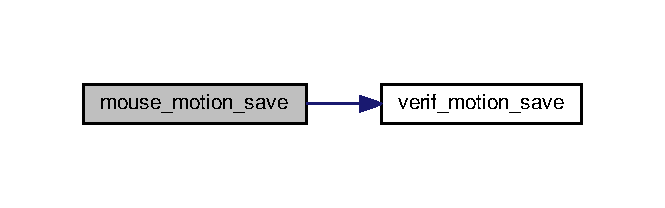
\includegraphics[width=319pt]{save_8c_a26ae7b755f8291e47249e059641a1cb5_cgraph}
\end{center}
\end{figure}




Here is the caller graph for this function\+:
\nopagebreak
\begin{figure}[H]
\begin{center}
\leavevmode
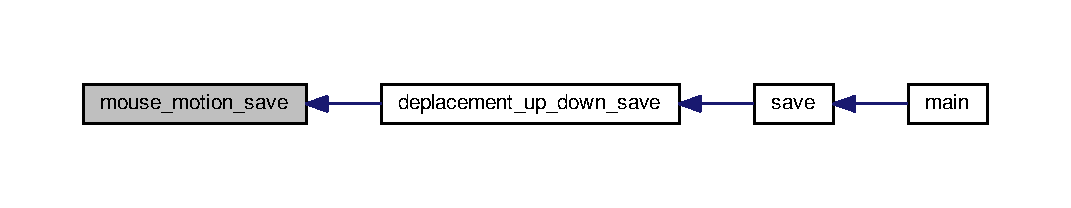
\includegraphics[width=350pt]{save_8c_a26ae7b755f8291e47249e059641a1cb5_icgraph}
\end{center}
\end{figure}


\index{save.\+c@{save.\+c}!mouvement@{mouvement}}
\index{mouvement@{mouvement}!save.\+c@{save.\+c}}
\subsubsection[{\texorpdfstring{mouvement(personnage $\ast$c)}{mouvement(personnage *c)}}]{\setlength{\rightskip}{0pt plus 5cm}void mouvement (
\begin{DoxyParamCaption}
\item[{{\bf personnage} $\ast$}]{c}
\end{DoxyParamCaption}
)}\hypertarget{save_8c_a936a0790f87300c4d50a1fe7959875f5}{}\label{save_8c_a936a0790f87300c4d50a1fe7959875f5}


to move hero 


\begin{DoxyParams}{Parameters}
{\em c=personnage} & \\
\hline
\end{DoxyParams}
\begin{DoxyReturn}{Returns}
nothing 
\end{DoxyReturn}


Here is the caller graph for this function\+:\nopagebreak
\begin{figure}[H]
\begin{center}
\leavevmode
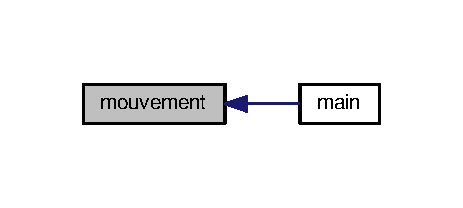
\includegraphics[width=222pt]{save_8c_a936a0790f87300c4d50a1fe7959875f5_icgraph}
\end{center}
\end{figure}


\index{save.\+c@{save.\+c}!mvm\+\_\+alea\+\_\+enemi@{mvm\+\_\+alea\+\_\+enemi}}
\index{mvm\+\_\+alea\+\_\+enemi@{mvm\+\_\+alea\+\_\+enemi}!save.\+c@{save.\+c}}
\subsubsection[{\texorpdfstring{mvm\+\_\+alea\+\_\+enemi(ennemi $\ast$e)}{mvm_alea_enemi(ennemi *e)}}]{\setlength{\rightskip}{0pt plus 5cm}void mvm\+\_\+alea\+\_\+enemi (
\begin{DoxyParamCaption}
\item[{{\bf ennemi} $\ast$}]{e}
\end{DoxyParamCaption}
)}\hypertarget{save_8c_a5b88fedc1de2481522fa32569e5b7393}{}\label{save_8c_a5b88fedc1de2481522fa32569e5b7393}




 

to move ennemy 
\begin{DoxyParams}{Parameters}
{\em e=ennemi} & \\
\hline
\end{DoxyParams}
\begin{DoxyReturn}{Returns}
nothing 
\end{DoxyReturn}


Here is the caller graph for this function\+:\nopagebreak
\begin{figure}[H]
\begin{center}
\leavevmode
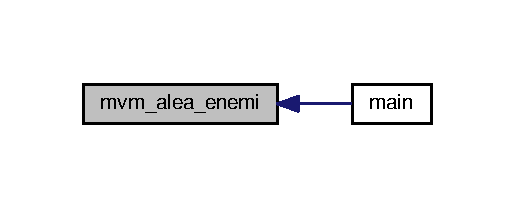
\includegraphics[width=247pt]{save_8c_a5b88fedc1de2481522fa32569e5b7393_icgraph}
\end{center}
\end{figure}


\index{save.\+c@{save.\+c}!save@{save}}
\index{save@{save}!save.\+c@{save.\+c}}
\subsubsection[{\texorpdfstring{save(\+S\+D\+L\+\_\+\+Surface $\ast$screen, S\+D\+L\+\_\+\+Event event, int $\ast$curseur, Objet sauv, Objet sauvn, Objet sauvy, Mix\+\_\+\+Chunk $\ast$effect, personnage c1, personnage c2, background b, char $\ast$file, ennemi e, int niveau, int $\ast$go)}{save(SDL_Surface *screen, SDL_Event event, int *curseur, Objet sauv, Objet sauvn, Objet sauvy, Mix_Chunk *effect, personnage c1, personnage c2, background b, char *file, ennemi e, int niveau, int *go)}}]{\setlength{\rightskip}{0pt plus 5cm}int save (
\begin{DoxyParamCaption}
\item[{S\+D\+L\+\_\+\+Surface $\ast$}]{screen, }
\item[{S\+D\+L\+\_\+\+Event}]{event, }
\item[{int $\ast$}]{curseur, }
\item[{{\bf Objet}}]{sauv, }
\item[{{\bf Objet}}]{sauvn, }
\item[{{\bf Objet}}]{sauvy, }
\item[{Mix\+\_\+\+Chunk $\ast$}]{effect, }
\item[{{\bf personnage}}]{c1, }
\item[{{\bf personnage}}]{c2, }
\item[{{\bf background}}]{b, }
\item[{char $\ast$}]{file, }
\item[{{\bf ennemi}}]{e, }
\item[{int}]{niveau, }
\item[{int $\ast$}]{go}
\end{DoxyParamCaption}
)}\hypertarget{save_8c_a34e892752d1de82a8306307f2e7dbfb7}{}\label{save_8c_a34e892752d1de82a8306307f2e7dbfb7}


to save game 


\begin{DoxyParams}{Parameters}
{\em screen} & \\
\hline
{\em event} & \\
\hline
{\em curseur} & \\
\hline
{\em sauv} & \\
\hline
{\em sauvn} & \\
\hline
{\em sauvy} & \\
\hline
{\em effect} & \\
\hline
{\em c1=personnage} & 1 \\
\hline
{\em c2=personnage} & 2 \\
\hline
{\em b=background} & \\
\hline
{\em file} & \\
\hline
{\em e=ennemy} & \\
\hline
{\em niveau} & \\
\hline
{\em go} & \\
\hline
{\em c=personnage} & \\
\hline
\end{DoxyParams}
\begin{DoxyReturn}{Returns}
nothing 
\end{DoxyReturn}


Here is the call graph for this function\+:
\nopagebreak
\begin{figure}[H]
\begin{center}
\leavevmode
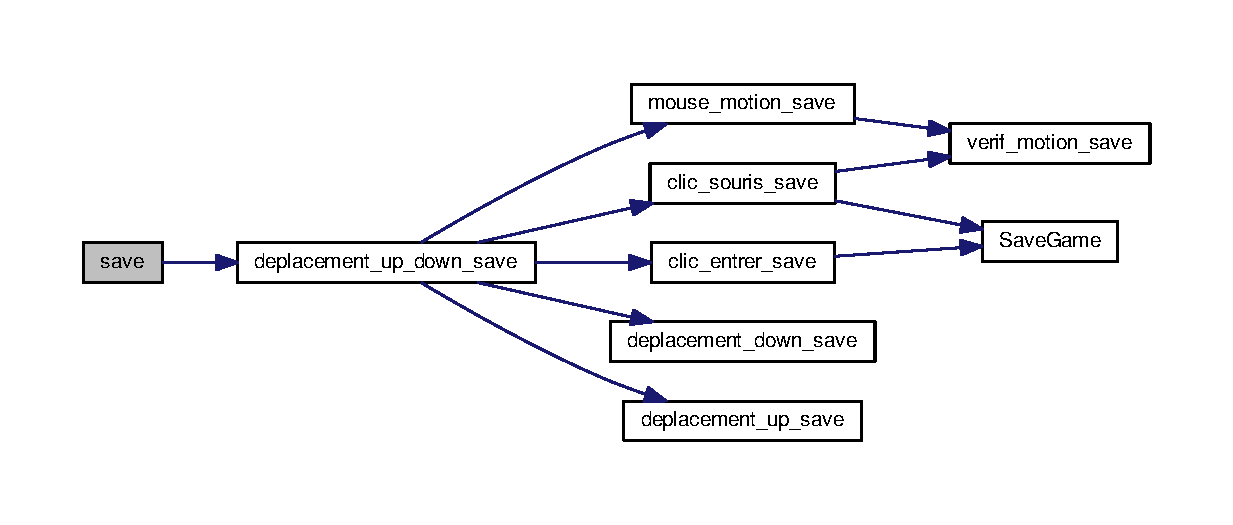
\includegraphics[width=350pt]{save_8c_a34e892752d1de82a8306307f2e7dbfb7_cgraph}
\end{center}
\end{figure}




Here is the caller graph for this function\+:
\nopagebreak
\begin{figure}[H]
\begin{center}
\leavevmode
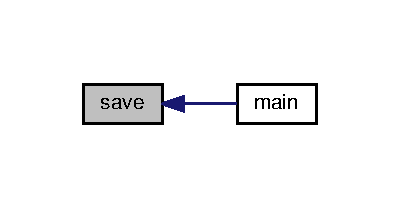
\includegraphics[width=192pt]{save_8c_a34e892752d1de82a8306307f2e7dbfb7_icgraph}
\end{center}
\end{figure}


\index{save.\+c@{save.\+c}!Save\+Game@{Save\+Game}}
\index{Save\+Game@{Save\+Game}!save.\+c@{save.\+c}}
\subsubsection[{\texorpdfstring{Save\+Game(personnage c1, personnage c2, background b, char $\ast$file, ennemi e, int niveau)}{SaveGame(personnage c1, personnage c2, background b, char *file, ennemi e, int niveau)}}]{\setlength{\rightskip}{0pt plus 5cm}void Save\+Game (
\begin{DoxyParamCaption}
\item[{{\bf personnage}}]{c1, }
\item[{{\bf personnage}}]{c2, }
\item[{{\bf background}}]{b, }
\item[{char $\ast$}]{file, }
\item[{{\bf ennemi}}]{e, }
\item[{int}]{niveau}
\end{DoxyParamCaption}
)}\hypertarget{save_8c_a30a06a7282f7de8937717af0b47b31cb}{}\label{save_8c_a30a06a7282f7de8937717af0b47b31cb}


to save game 


\begin{DoxyParams}{Parameters}
{\em c1=personnage1} & \\
\hline
{\em c2=personnage2} & \\
\hline
{\em b=background} & \\
\hline
{\em file} & \\
\hline
{\em e=ennemy} & \\
\hline
{\em niveau} & \\
\hline
\end{DoxyParams}
\begin{DoxyReturn}{Returns}
nothing 
\end{DoxyReturn}


Here is the caller graph for this function\+:
\nopagebreak
\begin{figure}[H]
\begin{center}
\leavevmode
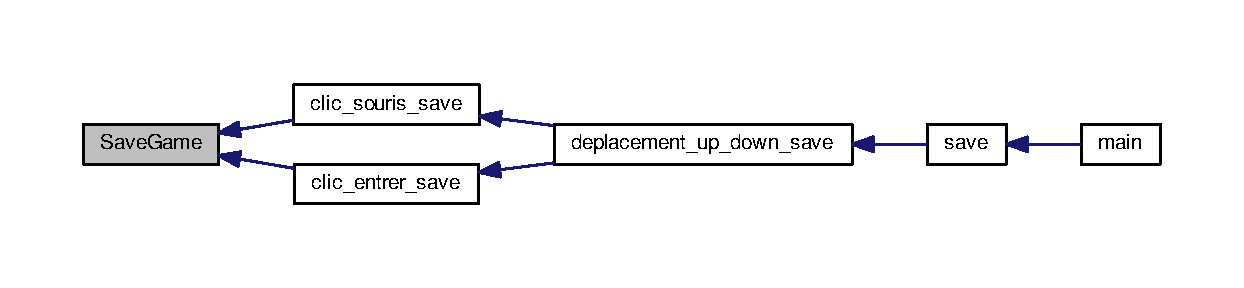
\includegraphics[width=350pt]{save_8c_a30a06a7282f7de8937717af0b47b31cb_icgraph}
\end{center}
\end{figure}


\index{save.\+c@{save.\+c}!verif\+\_\+motion\+\_\+save@{verif\+\_\+motion\+\_\+save}}
\index{verif\+\_\+motion\+\_\+save@{verif\+\_\+motion\+\_\+save}!save.\+c@{save.\+c}}
\subsubsection[{\texorpdfstring{verif\+\_\+motion\+\_\+save(\+S\+D\+L\+\_\+\+Event event, Objet surface)}{verif_motion_save(SDL_Event event, Objet surface)}}]{\setlength{\rightskip}{0pt plus 5cm}int verif\+\_\+motion\+\_\+save (
\begin{DoxyParamCaption}
\item[{S\+D\+L\+\_\+\+Event}]{event, }
\item[{{\bf Objet}}]{surface}
\end{DoxyParamCaption}
)}\hypertarget{save_8c_a323063e0b0a6c01cd3f01617e0df1d6e}{}\label{save_8c_a323063e0b0a6c01cd3f01617e0df1d6e}


to verify mouse motion 


\begin{DoxyParams}{Parameters}
{\em surface} & \\
\hline
{\em event} & \\
\hline
\end{DoxyParams}
\begin{DoxyReturn}{Returns}
entier 
\end{DoxyReturn}


Here is the caller graph for this function\+:
\nopagebreak
\begin{figure}[H]
\begin{center}
\leavevmode
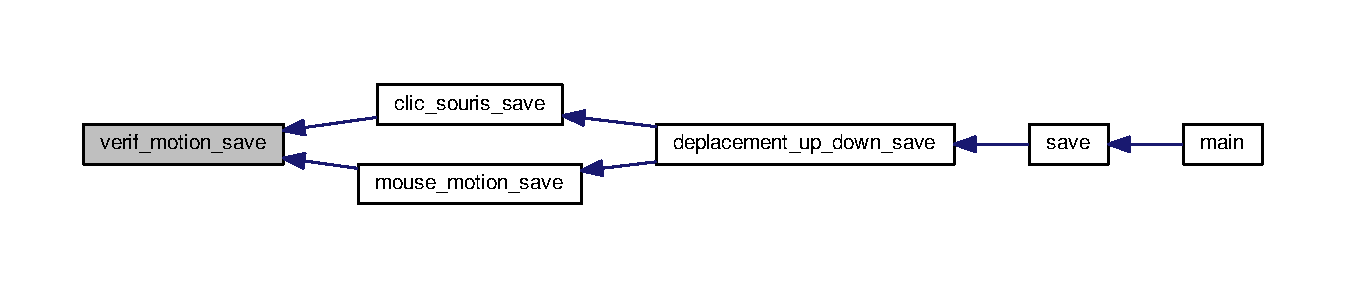
\includegraphics[width=350pt]{save_8c_a323063e0b0a6c01cd3f01617e0df1d6e_icgraph}
\end{center}
\end{figure}



\hypertarget{save_8h}{}\section{save.\+h File Reference}
\label{save_8h}\index{save.\+h@{save.\+h}}
{\ttfamily \#include $<$stdio.\+h$>$}\\*
{\ttfamily \#include $<$stdlib.\+h$>$}\\*
{\ttfamily \#include \char`\"{}S\+D\+L/\+S\+D\+L.\+h\char`\"{}}\\*
{\ttfamily \#include \char`\"{}S\+D\+L/\+S\+D\+L\+\_\+image.\+h\char`\"{}}\\*
{\ttfamily \#include \char`\"{}S\+D\+L/\+S\+D\+L\+\_\+mixer.\+h\char`\"{}}\\*
{\ttfamily \#include \char`\"{}S\+D\+L/\+S\+D\+L\+\_\+ttf.\+h\char`\"{}}\\*
Include dependency graph for save.\+h\+:\nopagebreak
\begin{figure}[H]
\begin{center}
\leavevmode
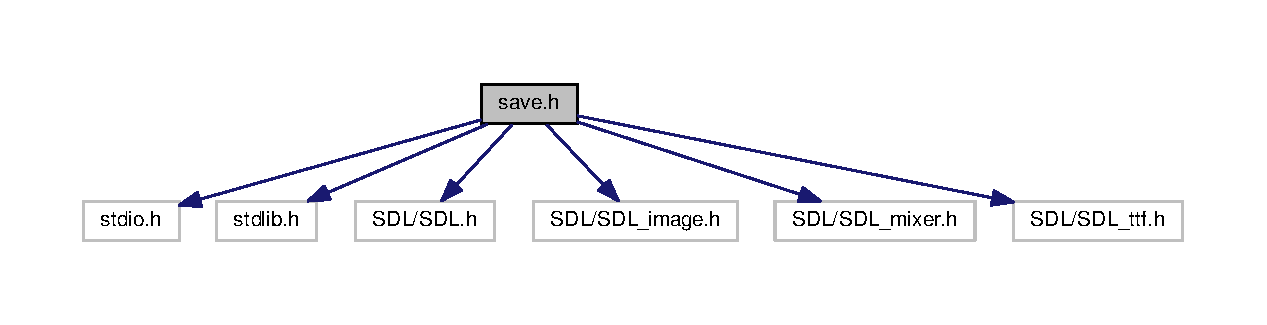
\includegraphics[width=350pt]{save_8h__incl}
\end{center}
\end{figure}
This graph shows which files directly or indirectly include this file\+:\nopagebreak
\begin{figure}[H]
\begin{center}
\leavevmode
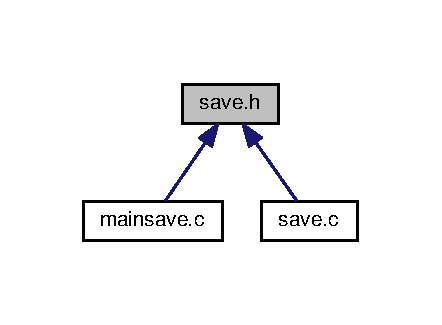
\includegraphics[width=212pt]{save_8h__dep__incl}
\end{center}
\end{figure}
\subsection*{Classes}
\begin{DoxyCompactItemize}
\item 
struct \hyperlink{structObjet}{Objet}
\item 
struct \hyperlink{structvie}{vie}
\begin{DoxyCompactList}\small\item\em struct for vie perso \end{DoxyCompactList}\item 
struct \hyperlink{structscore}{score}
\begin{DoxyCompactList}\small\item\em struct for score perso \end{DoxyCompactList}\item 
struct \hyperlink{structpersonnage}{personnage}
\begin{DoxyCompactList}\small\item\em struct for perso \end{DoxyCompactList}\item 
struct \hyperlink{structennemi}{ennemi}
\item 
struct \hyperlink{structbackground}{background}
\begin{DoxyCompactList}\small\item\em struct for background \end{DoxyCompactList}\end{DoxyCompactItemize}
\subsection*{Typedefs}
\begin{DoxyCompactItemize}
\item 
typedef struct \hyperlink{structvie}{vie} \hyperlink{save_8h_a5a50eadb578d4b4b9db54fdffc9b3c48}{vie}
\item 
typedef struct \hyperlink{structscore}{score} \hyperlink{save_8h_a1240ca29fa6f99334b17271ea026bc91}{score}
\item 
typedef struct \hyperlink{structpersonnage}{personnage} \hyperlink{save_8h_a22ea6c21be7b6540d95f47b6ad40ffa6}{personnage}
\item 
typedef struct \hyperlink{structennemi}{ennemi} \hyperlink{save_8h_ab7eb9415b369de28d9a91182c35b6fab}{ennemi}
\end{DoxyCompactItemize}
\subsection*{Functions}
\begin{DoxyCompactItemize}
\item 
void \hyperlink{save_8h_a30a06a7282f7de8937717af0b47b31cb}{Save\+Game} (\hyperlink{structpersonnage}{personnage} c1, \hyperlink{structpersonnage}{personnage} c2, \hyperlink{structbackground}{background} b, char $\ast$file, \hyperlink{structennemi}{ennemi} e, int niveau)
\begin{DoxyCompactList}\small\item\em to save game \end{DoxyCompactList}\item 
void \hyperlink{save_8h_acb4f6e609d2abc8783d41104e804ebf6}{initialiser\+\_\+save} (\hyperlink{structObjet}{Objet} $\ast$sauv, \hyperlink{structObjet}{Objet} $\ast$sauvy, \hyperlink{structObjet}{Objet} $\ast$sauvn)
\begin{DoxyCompactList}\small\item\em pour initialiser le menu de save oui/non \end{DoxyCompactList}\item 
int \hyperlink{save_8h_a323063e0b0a6c01cd3f01617e0df1d6e}{verif\+\_\+motion\+\_\+save} (S\+D\+L\+\_\+\+Event event, \hyperlink{structObjet}{Objet} surface)
\begin{DoxyCompactList}\small\item\em to verify mouse motion \end{DoxyCompactList}\item 
void \hyperlink{save_8h_a6897cc2439ee8a56c0d55f5e17bcd4dc}{clic\+\_\+souris\+\_\+save} (S\+D\+L\+\_\+\+Surface $\ast$screen, S\+D\+L\+\_\+\+Event event, int curseur, \hyperlink{structObjet}{Objet} sauvn, \hyperlink{structObjet}{Objet} sauvy, \hyperlink{structpersonnage}{personnage} c1, \hyperlink{structpersonnage}{personnage} c2, \hyperlink{structbackground}{background} b, char $\ast$file, \hyperlink{structennemi}{ennemi} e, int niveau)
\begin{DoxyCompactList}\small\item\em clic avec souris dans le menu de save oui/non \end{DoxyCompactList}\item 
void \hyperlink{save_8h_acd785e84ec9a4180b7686e73da03dd26}{clic\+\_\+entrer\+\_\+save} (S\+D\+L\+\_\+\+Surface $\ast$screen, Mix\+\_\+\+Chunk $\ast$effect, int curseur, \hyperlink{structObjet}{Objet} sauvn, \hyperlink{structObjet}{Objet} sauvy, \hyperlink{structpersonnage}{personnage} c1, \hyperlink{structpersonnage}{personnage} c2, \hyperlink{structbackground}{background} b, char $\ast$file, \hyperlink{structennemi}{ennemi} e, int niveau)
\begin{DoxyCompactList}\small\item\em clic avec bouton entrer dans le menu de save oui/non \end{DoxyCompactList}\item 
void \hyperlink{save_8h_a26ae7b755f8291e47249e059641a1cb5}{mouse\+\_\+motion\+\_\+save} (S\+D\+L\+\_\+\+Surface $\ast$screen, S\+D\+L\+\_\+\+Event event, Mix\+\_\+\+Chunk $\ast$effect, int $\ast$curseur, \hyperlink{structObjet}{Objet} sauvn, \hyperlink{structObjet}{Objet} sauvy)
\begin{DoxyCompactList}\small\item\em mouse motion dans le menu de save oui/non \end{DoxyCompactList}\item 
void \hyperlink{save_8h_a7fcb6ded09f67d099c5ec72e874d2261}{deplacement\+\_\+down\+\_\+save} (S\+D\+L\+\_\+\+Surface $\ast$screen, Mix\+\_\+\+Chunk $\ast$effect, int $\ast$curseur, \hyperlink{structObjet}{Objet} sauvn, \hyperlink{structObjet}{Objet} sauvy)
\begin{DoxyCompactList}\small\item\em se deplacer vers le bas dans le menu de save oui/non \end{DoxyCompactList}\item 
void \hyperlink{save_8h_a3d9d3c3144b808484894caf3bdded4fe}{deplacement\+\_\+up\+\_\+save} (S\+D\+L\+\_\+\+Surface $\ast$screen, Mix\+\_\+\+Chunk $\ast$effect, int $\ast$curseur, \hyperlink{structObjet}{Objet} sauvn, \hyperlink{structObjet}{Objet} sauvy)
\begin{DoxyCompactList}\small\item\em se deplacer vers le haut dans le menu de save oui/non \end{DoxyCompactList}\item 
int \hyperlink{save_8h_ae98bea39bce363158739b999ebc38ceb}{deplacement\+\_\+up\+\_\+down\+\_\+save} (S\+D\+L\+\_\+\+Surface $\ast$screen, S\+D\+L\+\_\+\+Event event, int $\ast$curseur, \hyperlink{structObjet}{Objet} sauvn, \hyperlink{structObjet}{Objet} sauvy, Mix\+\_\+\+Chunk $\ast$effect, int $\ast$go, \hyperlink{structpersonnage}{personnage} c1, \hyperlink{structpersonnage}{personnage} c2, \hyperlink{structbackground}{background} b, char $\ast$file, \hyperlink{structennemi}{ennemi} e, int niveau)
\begin{DoxyCompactList}\small\item\em se deplacer vers le bas et vers le haut dans le menu de save oui/non \end{DoxyCompactList}\item 
int \hyperlink{save_8h_a34e892752d1de82a8306307f2e7dbfb7}{save} (S\+D\+L\+\_\+\+Surface $\ast$screen, S\+D\+L\+\_\+\+Event event, int $\ast$curseur, \hyperlink{structObjet}{Objet} sauv, \hyperlink{structObjet}{Objet} sauvn, \hyperlink{structObjet}{Objet} sauvy, Mix\+\_\+\+Chunk $\ast$effect, \hyperlink{structpersonnage}{personnage} c1, \hyperlink{structpersonnage}{personnage} c2, \hyperlink{structbackground}{background} b, char $\ast$file, \hyperlink{structennemi}{ennemi} e, int niveau, int $\ast$go)
\begin{DoxyCompactList}\small\item\em to save game \end{DoxyCompactList}\item 
void \hyperlink{save_8h_a18376703725eb8a89b00df24948bee5f}{Load\+Game} (\hyperlink{structpersonnage}{personnage} $\ast$c1, \hyperlink{structpersonnage}{personnage} $\ast$c2, \hyperlink{structbackground}{background} $\ast$b, \hyperlink{structennemi}{ennemi} $\ast$e, int $\ast$niveau, S\+D\+L\+\_\+\+Surface $\ast$screen)
\begin{DoxyCompactList}\small\item\em to load game \end{DoxyCompactList}\item 
void \hyperlink{save_8h_a4ff1d38cf8edb29f59af5010d3e1b99e}{anim\+Enm} (\hyperlink{structennemi}{ennemi} $\ast$e, S\+D\+L\+\_\+\+Surface $\ast$screen)
\begin{DoxyCompactList}\small\item\em 

 \end{DoxyCompactList}\item 
void \hyperlink{save_8h_a449db8c266f1c795e8de1e9e9802f90b}{initialiserennemi} (\hyperlink{structennemi}{ennemi} $\ast$e)
\begin{DoxyCompactList}\small\item\em 

 \end{DoxyCompactList}\item 
void \hyperlink{save_8h_ad429715f94be9c05e0f873efd01f62ff}{freesurfaceennemi} (\hyperlink{structennemi}{ennemi} $\ast$e)
\begin{DoxyCompactList}\small\item\em 

 \end{DoxyCompactList}\item 
void \hyperlink{save_8h_ad7f4f5d982725341ae87b93b9b1a91fc}{affichage\+\_\+ennemi} (\hyperlink{structennemi}{ennemi} e, S\+D\+L\+\_\+\+Surface $\ast$screen)
\begin{DoxyCompactList}\small\item\em 

 \end{DoxyCompactList}\item 
void \hyperlink{save_8h_a5b88fedc1de2481522fa32569e5b7393}{mvm\+\_\+alea\+\_\+enemi} (\hyperlink{structennemi}{ennemi} $\ast$e)
\begin{DoxyCompactList}\small\item\em 

 \end{DoxyCompactList}\item 
\hyperlink{structpersonnage}{personnage} \hyperlink{save_8h_ad6b94a0d07757d441340deb27a5d26fe}{initiaperso} (\hyperlink{structpersonnage}{personnage} c)
\item 
\hyperlink{structpersonnage}{personnage} \hyperlink{save_8h_abc15402f1bc9be9a242db8d4f9403b4e}{initiaperso2} (\hyperlink{structpersonnage}{personnage} c)
\item 
\hyperlink{structpersonnage}{personnage} \hyperlink{save_8h_a8fd5cd633f844d0f565c513d966ecc2a}{initperso} (\hyperlink{structpersonnage}{personnage} c, int posx, int posy, int posw, int posh, int direction, int posviex, int posviey, int nbre\+\_\+de\+\_\+vie, int \hyperlink{structscore}{score}, int spritex, int spritey, int spritew, int spriteh, int numr, int numl, int posscorex, int posscorey, int velocity, int speed, int i)
\begin{DoxyCompactList}\small\item\em to initialize hero \end{DoxyCompactList}\item 
void \hyperlink{save_8h_a37690785871acb57ed11799088bec266}{animperso} (\hyperlink{structpersonnage}{personnage} $\ast$c, S\+D\+L\+\_\+\+Surface $\ast$screen)
\begin{DoxyCompactList}\small\item\em to animate hero \end{DoxyCompactList}\item 
void \hyperlink{save_8h_a4fcd9448740c67449649edb846515fae}{affichageperso} (\hyperlink{structpersonnage}{personnage} c, S\+D\+L\+\_\+\+Surface $\ast$screen)
\begin{DoxyCompactList}\small\item\em to display hero \end{DoxyCompactList}\item 
void \hyperlink{save_8h_a936a0790f87300c4d50a1fe7959875f5}{mouvement} (\hyperlink{structpersonnage}{personnage} $\ast$c)
\begin{DoxyCompactList}\small\item\em to move hero \end{DoxyCompactList}\item 
\hyperlink{structbackground}{background} \hyperlink{save_8h_a99dd96b8f84fbb251e26afc643890b8a}{initialiser\+\_\+background} (\hyperlink{structbackground}{background} b, int posx, int posy, int i)
\begin{DoxyCompactList}\small\item\em to initialize background \end{DoxyCompactList}\item 
\hyperlink{structennemi}{ennemi} \hyperlink{save_8h_a1237b088a523ece0f6f69491c5252e2e}{initialiser\+\_\+ennemi} (\hyperlink{structennemi}{ennemi} e, int eposition\+\_\+ennemix, int eposition\+\_\+ennemiy, int epos1x, int epos1y, int epos2x, int epos2y, int eposition\+\_\+spritex, int eposition\+\_\+spritey, int eposition\+\_\+spritew, int eposition\+\_\+spriteh, int edirection)
\begin{DoxyCompactList}\small\item\em to initialize ennemy \end{DoxyCompactList}\end{DoxyCompactItemize}


\subsection{Detailed Description}
Bouabker Arij \begin{DoxyDate}{Date}
Mai ,2020
\end{DoxyDate}
testing program for game saving and loading 

\subsection{Typedef Documentation}
\index{save.\+h@{save.\+h}!ennemi@{ennemi}}
\index{ennemi@{ennemi}!save.\+h@{save.\+h}}
\subsubsection[{\texorpdfstring{ennemi}{ennemi}}]{\setlength{\rightskip}{0pt plus 5cm}typedef struct {\bf ennemi} {\bf ennemi}}\hypertarget{save_8h_ab7eb9415b369de28d9a91182c35b6fab}{}\label{save_8h_ab7eb9415b369de28d9a91182c35b6fab}
\index{save.\+h@{save.\+h}!personnage@{personnage}}
\index{personnage@{personnage}!save.\+h@{save.\+h}}
\subsubsection[{\texorpdfstring{personnage}{personnage}}]{\setlength{\rightskip}{0pt plus 5cm}typedef struct {\bf personnage}  {\bf personnage}}\hypertarget{save_8h_a22ea6c21be7b6540d95f47b6ad40ffa6}{}\label{save_8h_a22ea6c21be7b6540d95f47b6ad40ffa6}
\index{save.\+h@{save.\+h}!score@{score}}
\index{score@{score}!save.\+h@{save.\+h}}
\subsubsection[{\texorpdfstring{score}{score}}]{\setlength{\rightskip}{0pt plus 5cm}typedef struct {\bf score} {\bf score}}\hypertarget{save_8h_a1240ca29fa6f99334b17271ea026bc91}{}\label{save_8h_a1240ca29fa6f99334b17271ea026bc91}
\index{save.\+h@{save.\+h}!vie@{vie}}
\index{vie@{vie}!save.\+h@{save.\+h}}
\subsubsection[{\texorpdfstring{vie}{vie}}]{\setlength{\rightskip}{0pt plus 5cm}typedef struct {\bf vie} {\bf vie}}\hypertarget{save_8h_a5a50eadb578d4b4b9db54fdffc9b3c48}{}\label{save_8h_a5a50eadb578d4b4b9db54fdffc9b3c48}


\subsection{Function Documentation}
\index{save.\+h@{save.\+h}!affichage\+\_\+ennemi@{affichage\+\_\+ennemi}}
\index{affichage\+\_\+ennemi@{affichage\+\_\+ennemi}!save.\+h@{save.\+h}}
\subsubsection[{\texorpdfstring{affichage\+\_\+ennemi(ennemi e, S\+D\+L\+\_\+\+Surface $\ast$screen)}{affichage_ennemi(ennemi e, SDL_Surface *screen)}}]{\setlength{\rightskip}{0pt plus 5cm}void affichage\+\_\+ennemi (
\begin{DoxyParamCaption}
\item[{{\bf ennemi}}]{e, }
\item[{S\+D\+L\+\_\+\+Surface $\ast$}]{screen}
\end{DoxyParamCaption}
)}\hypertarget{save_8h_ad7f4f5d982725341ae87b93b9b1a91fc}{}\label{save_8h_ad7f4f5d982725341ae87b93b9b1a91fc}




 

to display ennemy 
\begin{DoxyParams}{Parameters}
{\em screen} & \\
\hline
{\em e=ennemi} & \\
\hline
\end{DoxyParams}
\begin{DoxyReturn}{Returns}
nothing 
\end{DoxyReturn}


Here is the caller graph for this function\+:\nopagebreak
\begin{figure}[H]
\begin{center}
\leavevmode
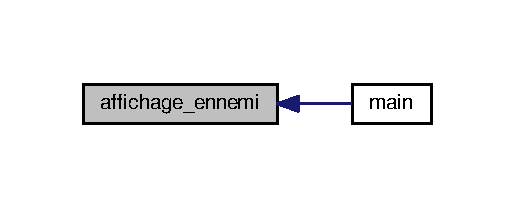
\includegraphics[width=247pt]{save_8h_ad7f4f5d982725341ae87b93b9b1a91fc_icgraph}
\end{center}
\end{figure}


\index{save.\+h@{save.\+h}!affichageperso@{affichageperso}}
\index{affichageperso@{affichageperso}!save.\+h@{save.\+h}}
\subsubsection[{\texorpdfstring{affichageperso(personnage c, S\+D\+L\+\_\+\+Surface $\ast$screen)}{affichageperso(personnage c, SDL_Surface *screen)}}]{\setlength{\rightskip}{0pt plus 5cm}void affichageperso (
\begin{DoxyParamCaption}
\item[{{\bf personnage}}]{c, }
\item[{S\+D\+L\+\_\+\+Surface $\ast$}]{screen}
\end{DoxyParamCaption}
)}\hypertarget{save_8h_a4fcd9448740c67449649edb846515fae}{}\label{save_8h_a4fcd9448740c67449649edb846515fae}


to display hero 


\begin{DoxyParams}{Parameters}
{\em c=personnage} & \\
\hline
{\em screen} & \\
\hline
\end{DoxyParams}
\begin{DoxyReturn}{Returns}
nothing 
\end{DoxyReturn}


Here is the call graph for this function\+:\nopagebreak
\begin{figure}[H]
\begin{center}
\leavevmode
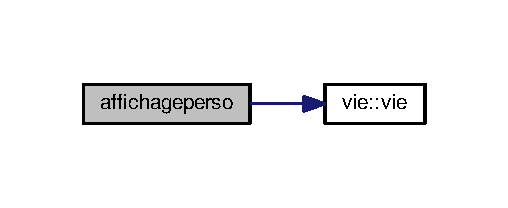
\includegraphics[width=244pt]{save_8h_a4fcd9448740c67449649edb846515fae_cgraph}
\end{center}
\end{figure}




Here is the caller graph for this function\+:\nopagebreak
\begin{figure}[H]
\begin{center}
\leavevmode
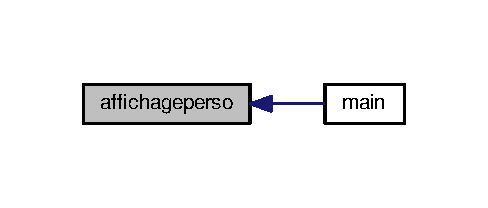
\includegraphics[width=234pt]{save_8h_a4fcd9448740c67449649edb846515fae_icgraph}
\end{center}
\end{figure}


\index{save.\+h@{save.\+h}!anim\+Enm@{anim\+Enm}}
\index{anim\+Enm@{anim\+Enm}!save.\+h@{save.\+h}}
\subsubsection[{\texorpdfstring{anim\+Enm(ennemi $\ast$e, S\+D\+L\+\_\+\+Surface $\ast$screen)}{animEnm(ennemi *e, SDL_Surface *screen)}}]{\setlength{\rightskip}{0pt plus 5cm}void anim\+Enm (
\begin{DoxyParamCaption}
\item[{{\bf ennemi} $\ast$}]{e, }
\item[{S\+D\+L\+\_\+\+Surface $\ast$}]{screen}
\end{DoxyParamCaption}
)}\hypertarget{save_8h_a4ff1d38cf8edb29f59af5010d3e1b99e}{}\label{save_8h_a4ff1d38cf8edb29f59af5010d3e1b99e}




 

to animate ennemy 
\begin{DoxyParams}{Parameters}
{\em screen} & \\
\hline
{\em e=ennemi} & \\
\hline
\end{DoxyParams}
\begin{DoxyReturn}{Returns}
nothing 
\end{DoxyReturn}
\index{save.\+h@{save.\+h}!animperso@{animperso}}
\index{animperso@{animperso}!save.\+h@{save.\+h}}
\subsubsection[{\texorpdfstring{animperso(personnage $\ast$c, S\+D\+L\+\_\+\+Surface $\ast$screen)}{animperso(personnage *c, SDL_Surface *screen)}}]{\setlength{\rightskip}{0pt plus 5cm}void animperso (
\begin{DoxyParamCaption}
\item[{{\bf personnage} $\ast$}]{c, }
\item[{S\+D\+L\+\_\+\+Surface $\ast$}]{screen}
\end{DoxyParamCaption}
)}\hypertarget{save_8h_a37690785871acb57ed11799088bec266}{}\label{save_8h_a37690785871acb57ed11799088bec266}


to animate hero 


\begin{DoxyParams}{Parameters}
{\em c=personnage} & \\
\hline
{\em screen} & \\
\hline
\end{DoxyParams}
\begin{DoxyReturn}{Returns}
nothing 
\end{DoxyReturn}


Here is the caller graph for this function\+:\nopagebreak
\begin{figure}[H]
\begin{center}
\leavevmode
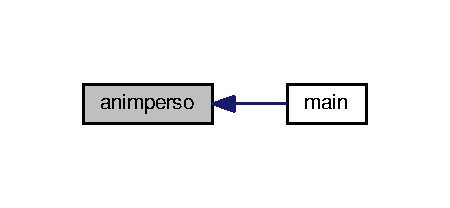
\includegraphics[width=216pt]{save_8h_a37690785871acb57ed11799088bec266_icgraph}
\end{center}
\end{figure}


\index{save.\+h@{save.\+h}!clic\+\_\+entrer\+\_\+save@{clic\+\_\+entrer\+\_\+save}}
\index{clic\+\_\+entrer\+\_\+save@{clic\+\_\+entrer\+\_\+save}!save.\+h@{save.\+h}}
\subsubsection[{\texorpdfstring{clic\+\_\+entrer\+\_\+save(\+S\+D\+L\+\_\+\+Surface $\ast$screen, Mix\+\_\+\+Chunk $\ast$effect, int curseur, Objet sauvn, Objet sauvy, personnage c1, personnage c2, background b, char $\ast$file, ennemi e, int niveau)}{clic_entrer_save(SDL_Surface *screen, Mix_Chunk *effect, int curseur, Objet sauvn, Objet sauvy, personnage c1, personnage c2, background b, char *file, ennemi e, int niveau)}}]{\setlength{\rightskip}{0pt plus 5cm}void clic\+\_\+entrer\+\_\+save (
\begin{DoxyParamCaption}
\item[{S\+D\+L\+\_\+\+Surface $\ast$}]{screen, }
\item[{Mix\+\_\+\+Chunk $\ast$}]{effect, }
\item[{int}]{curseur, }
\item[{{\bf Objet}}]{sauvn, }
\item[{{\bf Objet}}]{sauvy, }
\item[{{\bf personnage}}]{c1, }
\item[{{\bf personnage}}]{c2, }
\item[{{\bf background}}]{b, }
\item[{char $\ast$}]{file, }
\item[{{\bf ennemi}}]{e, }
\item[{int}]{niveau}
\end{DoxyParamCaption}
)}\hypertarget{save_8h_acd785e84ec9a4180b7686e73da03dd26}{}\label{save_8h_acd785e84ec9a4180b7686e73da03dd26}


clic avec bouton entrer dans le menu de save oui/non 


\begin{DoxyParams}{Parameters}
{\em screen} & \\
\hline
{\em effect} & \\
\hline
{\em curseur} & \\
\hline
{\em sauvy} & \\
\hline
{\em sauvn} & \\
\hline
{\em c1=personnage} & 1 \\
\hline
{\em c2=personnage} & 2 \\
\hline
{\em b=background} & \\
\hline
{\em file} & \\
\hline
{\em e=ennemy} & \\
\hline
{\em niveau} & \\
\hline
\end{DoxyParams}
\begin{DoxyReturn}{Returns}
nothing 
\end{DoxyReturn}


Here is the call graph for this function\+:\nopagebreak
\begin{figure}[H]
\begin{center}
\leavevmode
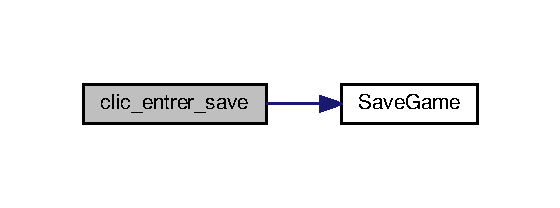
\includegraphics[width=269pt]{save_8h_acd785e84ec9a4180b7686e73da03dd26_cgraph}
\end{center}
\end{figure}




Here is the caller graph for this function\+:
\nopagebreak
\begin{figure}[H]
\begin{center}
\leavevmode
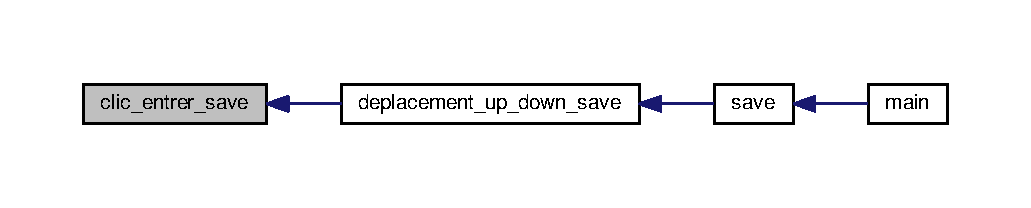
\includegraphics[width=350pt]{save_8h_acd785e84ec9a4180b7686e73da03dd26_icgraph}
\end{center}
\end{figure}


\index{save.\+h@{save.\+h}!clic\+\_\+souris\+\_\+save@{clic\+\_\+souris\+\_\+save}}
\index{clic\+\_\+souris\+\_\+save@{clic\+\_\+souris\+\_\+save}!save.\+h@{save.\+h}}
\subsubsection[{\texorpdfstring{clic\+\_\+souris\+\_\+save(\+S\+D\+L\+\_\+\+Surface $\ast$screen, S\+D\+L\+\_\+\+Event event, int curseur, Objet sauvn, Objet sauvy, personnage c1, personnage c2, background b, char $\ast$file, ennemi e, int niveau)}{clic_souris_save(SDL_Surface *screen, SDL_Event event, int curseur, Objet sauvn, Objet sauvy, personnage c1, personnage c2, background b, char *file, ennemi e, int niveau)}}]{\setlength{\rightskip}{0pt plus 5cm}void clic\+\_\+souris\+\_\+save (
\begin{DoxyParamCaption}
\item[{S\+D\+L\+\_\+\+Surface $\ast$}]{screen, }
\item[{S\+D\+L\+\_\+\+Event}]{event, }
\item[{int}]{curseur, }
\item[{{\bf Objet}}]{sauvn, }
\item[{{\bf Objet}}]{sauvy, }
\item[{{\bf personnage}}]{c1, }
\item[{{\bf personnage}}]{c2, }
\item[{{\bf background}}]{b, }
\item[{char $\ast$}]{file, }
\item[{{\bf ennemi}}]{e, }
\item[{int}]{niveau}
\end{DoxyParamCaption}
)}\hypertarget{save_8h_a6897cc2439ee8a56c0d55f5e17bcd4dc}{}\label{save_8h_a6897cc2439ee8a56c0d55f5e17bcd4dc}


clic avec souris dans le menu de save oui/non 


\begin{DoxyParams}{Parameters}
{\em screen} & \\
\hline
{\em event} & \\
\hline
{\em curseur} & \\
\hline
{\em sauvy} & \\
\hline
{\em sauvn} & \\
\hline
{\em c1=personnage} & 1 \\
\hline
{\em c2=personnage} & 2 \\
\hline
{\em b=background} & \\
\hline
{\em file} & \\
\hline
{\em e=ennemy} & \\
\hline
{\em niveau} & \\
\hline
\end{DoxyParams}
\begin{DoxyReturn}{Returns}
nothing 
\end{DoxyReturn}


Here is the call graph for this function\+:\nopagebreak
\begin{figure}[H]
\begin{center}
\leavevmode
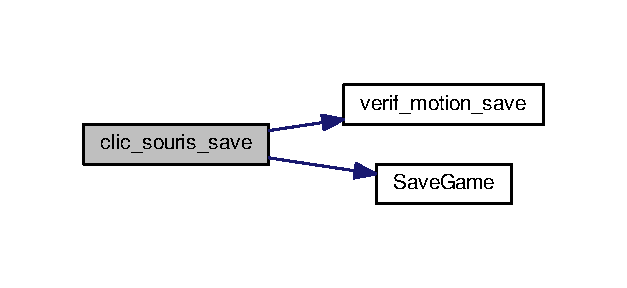
\includegraphics[width=301pt]{save_8h_a6897cc2439ee8a56c0d55f5e17bcd4dc_cgraph}
\end{center}
\end{figure}




Here is the caller graph for this function\+:
\nopagebreak
\begin{figure}[H]
\begin{center}
\leavevmode
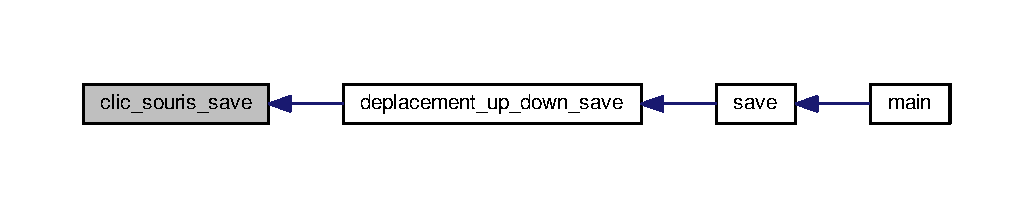
\includegraphics[width=350pt]{save_8h_a6897cc2439ee8a56c0d55f5e17bcd4dc_icgraph}
\end{center}
\end{figure}


\index{save.\+h@{save.\+h}!deplacement\+\_\+down\+\_\+save@{deplacement\+\_\+down\+\_\+save}}
\index{deplacement\+\_\+down\+\_\+save@{deplacement\+\_\+down\+\_\+save}!save.\+h@{save.\+h}}
\subsubsection[{\texorpdfstring{deplacement\+\_\+down\+\_\+save(\+S\+D\+L\+\_\+\+Surface $\ast$screen, Mix\+\_\+\+Chunk $\ast$effect, int $\ast$curseur, Objet sauvn, Objet sauvy)}{deplacement_down_save(SDL_Surface *screen, Mix_Chunk *effect, int *curseur, Objet sauvn, Objet sauvy)}}]{\setlength{\rightskip}{0pt plus 5cm}void deplacement\+\_\+down\+\_\+save (
\begin{DoxyParamCaption}
\item[{S\+D\+L\+\_\+\+Surface $\ast$}]{screen, }
\item[{Mix\+\_\+\+Chunk $\ast$}]{effect, }
\item[{int $\ast$}]{curseur, }
\item[{{\bf Objet}}]{sauvn, }
\item[{{\bf Objet}}]{sauvy}
\end{DoxyParamCaption}
)}\hypertarget{save_8h_a7fcb6ded09f67d099c5ec72e874d2261}{}\label{save_8h_a7fcb6ded09f67d099c5ec72e874d2261}


se deplacer vers le bas dans le menu de save oui/non 


\begin{DoxyParams}{Parameters}
{\em screen} & \\
\hline
{\em sauvn} & \\
\hline
{\em sauvy} & \\
\hline
{\em curseur} & \\
\hline
{\em effect} & \\
\hline
\end{DoxyParams}
\begin{DoxyReturn}{Returns}
nothing 
\end{DoxyReturn}


Here is the caller graph for this function\+:
\nopagebreak
\begin{figure}[H]
\begin{center}
\leavevmode
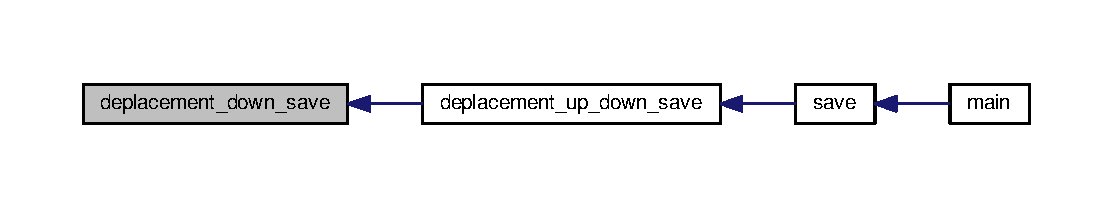
\includegraphics[width=350pt]{save_8h_a7fcb6ded09f67d099c5ec72e874d2261_icgraph}
\end{center}
\end{figure}


\index{save.\+h@{save.\+h}!deplacement\+\_\+up\+\_\+down\+\_\+save@{deplacement\+\_\+up\+\_\+down\+\_\+save}}
\index{deplacement\+\_\+up\+\_\+down\+\_\+save@{deplacement\+\_\+up\+\_\+down\+\_\+save}!save.\+h@{save.\+h}}
\subsubsection[{\texorpdfstring{deplacement\+\_\+up\+\_\+down\+\_\+save(\+S\+D\+L\+\_\+\+Surface $\ast$screen, S\+D\+L\+\_\+\+Event event, int $\ast$curseur, Objet sauvn, Objet sauvy, Mix\+\_\+\+Chunk $\ast$effect, int $\ast$go, personnage c1, personnage c2, background b, char $\ast$file, ennemi e, int niveau)}{deplacement_up_down_save(SDL_Surface *screen, SDL_Event event, int *curseur, Objet sauvn, Objet sauvy, Mix_Chunk *effect, int *go, personnage c1, personnage c2, background b, char *file, ennemi e, int niveau)}}]{\setlength{\rightskip}{0pt plus 5cm}int deplacement\+\_\+up\+\_\+down\+\_\+save (
\begin{DoxyParamCaption}
\item[{S\+D\+L\+\_\+\+Surface $\ast$}]{screen, }
\item[{S\+D\+L\+\_\+\+Event}]{event, }
\item[{int $\ast$}]{curseur, }
\item[{{\bf Objet}}]{sauvn, }
\item[{{\bf Objet}}]{sauvy, }
\item[{Mix\+\_\+\+Chunk $\ast$}]{effect, }
\item[{int $\ast$}]{go, }
\item[{{\bf personnage}}]{c1, }
\item[{{\bf personnage}}]{c2, }
\item[{{\bf background}}]{b, }
\item[{char $\ast$}]{file, }
\item[{{\bf ennemi}}]{e, }
\item[{int}]{niveau}
\end{DoxyParamCaption}
)}\hypertarget{save_8h_ae98bea39bce363158739b999ebc38ceb}{}\label{save_8h_ae98bea39bce363158739b999ebc38ceb}


se deplacer vers le bas et vers le haut dans le menu de save oui/non 


\begin{DoxyParams}{Parameters}
{\em screen} & \\
\hline
{\em event} & \\
\hline
{\em curseur} & \\
\hline
{\em sauv} & \\
\hline
{\em sauvn} & \\
\hline
{\em sauvy} & \\
\hline
{\em effect} & \\
\hline
{\em c1=personnage} & 1 \\
\hline
{\em c2=personnage} & 2 \\
\hline
{\em b=background} & \\
\hline
{\em file} & \\
\hline
{\em e=ennemy} & \\
\hline
{\em niveau} & \\
\hline
{\em go} & \\
\hline
{\em c=personnage} & \\
\hline
\end{DoxyParams}
\begin{DoxyReturn}{Returns}
nothing 
\end{DoxyReturn}


Here is the call graph for this function\+:
\nopagebreak
\begin{figure}[H]
\begin{center}
\leavevmode
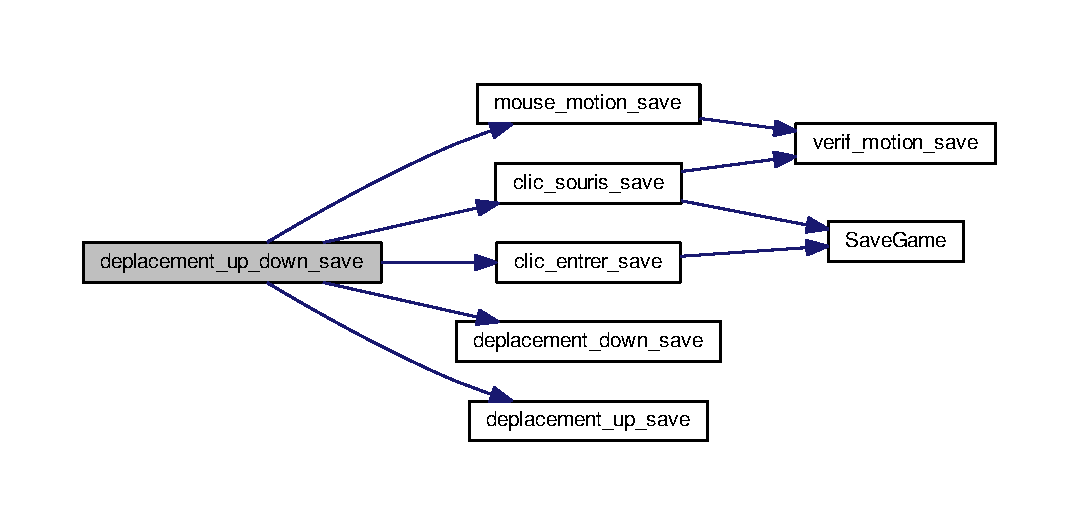
\includegraphics[width=350pt]{save_8h_ae98bea39bce363158739b999ebc38ceb_cgraph}
\end{center}
\end{figure}




Here is the caller graph for this function\+:
\nopagebreak
\begin{figure}[H]
\begin{center}
\leavevmode
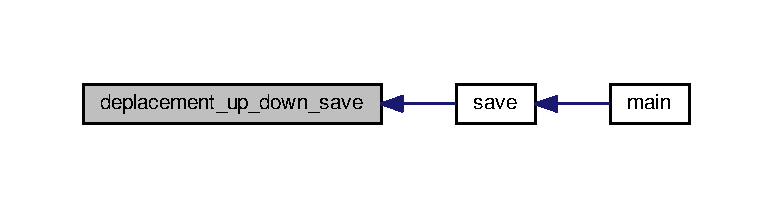
\includegraphics[width=350pt]{save_8h_ae98bea39bce363158739b999ebc38ceb_icgraph}
\end{center}
\end{figure}


\index{save.\+h@{save.\+h}!deplacement\+\_\+up\+\_\+save@{deplacement\+\_\+up\+\_\+save}}
\index{deplacement\+\_\+up\+\_\+save@{deplacement\+\_\+up\+\_\+save}!save.\+h@{save.\+h}}
\subsubsection[{\texorpdfstring{deplacement\+\_\+up\+\_\+save(\+S\+D\+L\+\_\+\+Surface $\ast$screen, Mix\+\_\+\+Chunk $\ast$effect, int $\ast$curseur, Objet sauvn, Objet sauvy)}{deplacement_up_save(SDL_Surface *screen, Mix_Chunk *effect, int *curseur, Objet sauvn, Objet sauvy)}}]{\setlength{\rightskip}{0pt plus 5cm}void deplacement\+\_\+up\+\_\+save (
\begin{DoxyParamCaption}
\item[{S\+D\+L\+\_\+\+Surface $\ast$}]{screen, }
\item[{Mix\+\_\+\+Chunk $\ast$}]{effect, }
\item[{int $\ast$}]{curseur, }
\item[{{\bf Objet}}]{sauvn, }
\item[{{\bf Objet}}]{sauvy}
\end{DoxyParamCaption}
)}\hypertarget{save_8h_a3d9d3c3144b808484894caf3bdded4fe}{}\label{save_8h_a3d9d3c3144b808484894caf3bdded4fe}


se deplacer vers le haut dans le menu de save oui/non 


\begin{DoxyParams}{Parameters}
{\em screen} & \\
\hline
{\em curseur} & \\
\hline
{\em sauvn} & \\
\hline
{\em sauvy} & \\
\hline
{\em effect} & \\
\hline
\end{DoxyParams}
\begin{DoxyReturn}{Returns}
nothing 
\end{DoxyReturn}


Here is the caller graph for this function\+:
\nopagebreak
\begin{figure}[H]
\begin{center}
\leavevmode
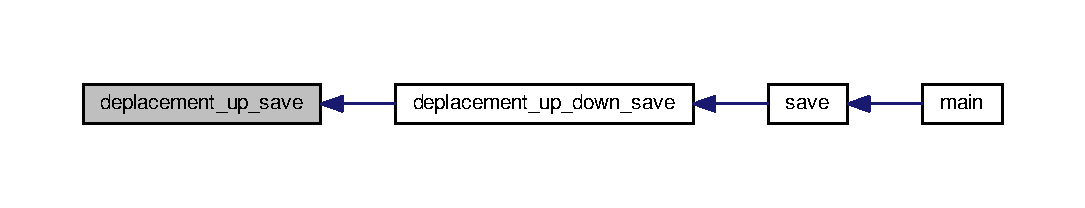
\includegraphics[width=350pt]{save_8h_a3d9d3c3144b808484894caf3bdded4fe_icgraph}
\end{center}
\end{figure}


\index{save.\+h@{save.\+h}!freesurfaceennemi@{freesurfaceennemi}}
\index{freesurfaceennemi@{freesurfaceennemi}!save.\+h@{save.\+h}}
\subsubsection[{\texorpdfstring{freesurfaceennemi(ennemi $\ast$e)}{freesurfaceennemi(ennemi *e)}}]{\setlength{\rightskip}{0pt plus 5cm}void freesurfaceennemi (
\begin{DoxyParamCaption}
\item[{{\bf ennemi} $\ast$}]{e}
\end{DoxyParamCaption}
)}\hypertarget{save_8h_ad429715f94be9c05e0f873efd01f62ff}{}\label{save_8h_ad429715f94be9c05e0f873efd01f62ff}




 

to free memory from ennemy 
\begin{DoxyParams}{Parameters}
{\em e=ennemi} & \\
\hline
\end{DoxyParams}
\begin{DoxyReturn}{Returns}
nothing 
\end{DoxyReturn}


Here is the caller graph for this function\+:\nopagebreak
\begin{figure}[H]
\begin{center}
\leavevmode
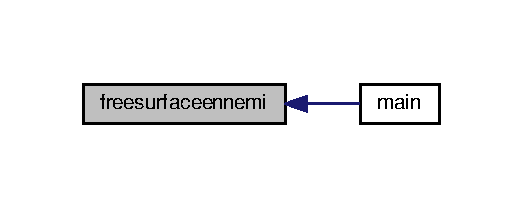
\includegraphics[width=251pt]{save_8h_ad429715f94be9c05e0f873efd01f62ff_icgraph}
\end{center}
\end{figure}


\index{save.\+h@{save.\+h}!initialiser\+\_\+background@{initialiser\+\_\+background}}
\index{initialiser\+\_\+background@{initialiser\+\_\+background}!save.\+h@{save.\+h}}
\subsubsection[{\texorpdfstring{initialiser\+\_\+background(background b, int posx, int posy, int i)}{initialiser_background(background b, int posx, int posy, int i)}}]{\setlength{\rightskip}{0pt plus 5cm}{\bf background} initialiser\+\_\+background (
\begin{DoxyParamCaption}
\item[{{\bf background}}]{b, }
\item[{int}]{posx, }
\item[{int}]{posy, }
\item[{int}]{i}
\end{DoxyParamCaption}
)}\hypertarget{save_8h_a99dd96b8f84fbb251e26afc643890b8a}{}\label{save_8h_a99dd96b8f84fbb251e26afc643890b8a}


to initialize background 

\begin{DoxyReturn}{Returns}
background 
\end{DoxyReturn}


Here is the caller graph for this function\+:\nopagebreak
\begin{figure}[H]
\begin{center}
\leavevmode
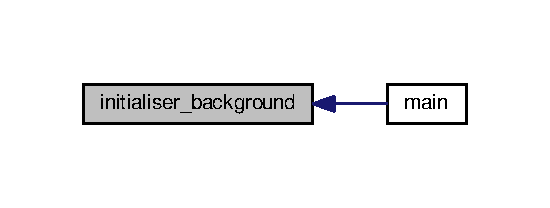
\includegraphics[width=264pt]{save_8h_a99dd96b8f84fbb251e26afc643890b8a_icgraph}
\end{center}
\end{figure}


\index{save.\+h@{save.\+h}!initialiser\+\_\+ennemi@{initialiser\+\_\+ennemi}}
\index{initialiser\+\_\+ennemi@{initialiser\+\_\+ennemi}!save.\+h@{save.\+h}}
\subsubsection[{\texorpdfstring{initialiser\+\_\+ennemi(ennemi e, int eposition\+\_\+ennemix, int eposition\+\_\+ennemiy, int epos1x, int epos1y, int epos2x, int epos2y, int eposition\+\_\+spritex, int eposition\+\_\+spritey, int eposition\+\_\+spritew, int eposition\+\_\+spriteh, int edirection)}{initialiser_ennemi(ennemi e, int eposition_ennemix, int eposition_ennemiy, int epos1x, int epos1y, int epos2x, int epos2y, int eposition_spritex, int eposition_spritey, int eposition_spritew, int eposition_spriteh, int edirection)}}]{\setlength{\rightskip}{0pt plus 5cm}{\bf ennemi} initialiser\+\_\+ennemi (
\begin{DoxyParamCaption}
\item[{{\bf ennemi}}]{e, }
\item[{int}]{eposition\+\_\+ennemix, }
\item[{int}]{eposition\+\_\+ennemiy, }
\item[{int}]{epos1x, }
\item[{int}]{epos1y, }
\item[{int}]{epos2x, }
\item[{int}]{epos2y, }
\item[{int}]{eposition\+\_\+spritex, }
\item[{int}]{eposition\+\_\+spritey, }
\item[{int}]{eposition\+\_\+spritew, }
\item[{int}]{eposition\+\_\+spriteh, }
\item[{int}]{edirection}
\end{DoxyParamCaption}
)}\hypertarget{save_8h_a1237b088a523ece0f6f69491c5252e2e}{}\label{save_8h_a1237b088a523ece0f6f69491c5252e2e}


to initialize ennemy 

\begin{DoxyReturn}{Returns}
ennemy 
\end{DoxyReturn}
\index{save.\+h@{save.\+h}!initialiser\+\_\+save@{initialiser\+\_\+save}}
\index{initialiser\+\_\+save@{initialiser\+\_\+save}!save.\+h@{save.\+h}}
\subsubsection[{\texorpdfstring{initialiser\+\_\+save(\+Objet $\ast$sauv, Objet $\ast$sauvy, Objet $\ast$sauvn)}{initialiser_save(Objet *sauv, Objet *sauvy, Objet *sauvn)}}]{\setlength{\rightskip}{0pt plus 5cm}void initialiser\+\_\+save (
\begin{DoxyParamCaption}
\item[{{\bf Objet} $\ast$}]{sauv, }
\item[{{\bf Objet} $\ast$}]{sauvy, }
\item[{{\bf Objet} $\ast$}]{sauvn}
\end{DoxyParamCaption}
)}\hypertarget{save_8h_acb4f6e609d2abc8783d41104e804ebf6}{}\label{save_8h_acb4f6e609d2abc8783d41104e804ebf6}


pour initialiser le menu de save oui/non 


\begin{DoxyParams}{Parameters}
{\em sauvy} & \\
\hline
{\em sauvn} & \\
\hline
{\em sauv} & \\
\hline
\end{DoxyParams}
\begin{DoxyReturn}{Returns}
nothing 
\end{DoxyReturn}


Here is the caller graph for this function\+:\nopagebreak
\begin{figure}[H]
\begin{center}
\leavevmode
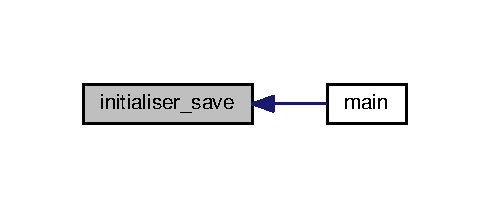
\includegraphics[width=235pt]{save_8h_acb4f6e609d2abc8783d41104e804ebf6_icgraph}
\end{center}
\end{figure}


\index{save.\+h@{save.\+h}!initialiserennemi@{initialiserennemi}}
\index{initialiserennemi@{initialiserennemi}!save.\+h@{save.\+h}}
\subsubsection[{\texorpdfstring{initialiserennemi(ennemi $\ast$e)}{initialiserennemi(ennemi *e)}}]{\setlength{\rightskip}{0pt plus 5cm}void initialiserennemi (
\begin{DoxyParamCaption}
\item[{{\bf ennemi} $\ast$}]{e}
\end{DoxyParamCaption}
)}\hypertarget{save_8h_a449db8c266f1c795e8de1e9e9802f90b}{}\label{save_8h_a449db8c266f1c795e8de1e9e9802f90b}




 

to initialize ennemy

to initialize ennemy 
\begin{DoxyParams}{Parameters}
{\em e=ennemi} & \\
\hline
\end{DoxyParams}
\begin{DoxyReturn}{Returns}
nothing

nothing
\end{DoxyReturn}




\begin{DoxyReturn}{Returns}
nothing 
\end{DoxyReturn}


Here is the caller graph for this function\+:\nopagebreak
\begin{figure}[H]
\begin{center}
\leavevmode
\includegraphics[width=240pt]{save_8h_a449db8c266f1c795e8de1e9e9802f90b_icgraph}
\end{center}
\end{figure}


\index{save.\+h@{save.\+h}!initiaperso@{initiaperso}}
\index{initiaperso@{initiaperso}!save.\+h@{save.\+h}}
\subsubsection[{\texorpdfstring{initiaperso(personnage c)}{initiaperso(personnage c)}}]{\setlength{\rightskip}{0pt plus 5cm}{\bf personnage} initiaperso (
\begin{DoxyParamCaption}
\item[{{\bf personnage}}]{c}
\end{DoxyParamCaption}
)}\hypertarget{save_8h_ad6b94a0d07757d441340deb27a5d26fe}{}\label{save_8h_ad6b94a0d07757d441340deb27a5d26fe}


Here is the call graph for this function\+:\nopagebreak
\begin{figure}[H]
\begin{center}
\leavevmode
\includegraphics[width=225pt]{save_8h_ad6b94a0d07757d441340deb27a5d26fe_cgraph}
\end{center}
\end{figure}




Here is the caller graph for this function\+:\nopagebreak
\begin{figure}[H]
\begin{center}
\leavevmode
\includegraphics[width=215pt]{save_8h_ad6b94a0d07757d441340deb27a5d26fe_icgraph}
\end{center}
\end{figure}


\index{save.\+h@{save.\+h}!initiaperso2@{initiaperso2}}
\index{initiaperso2@{initiaperso2}!save.\+h@{save.\+h}}
\subsubsection[{\texorpdfstring{initiaperso2(personnage c)}{initiaperso2(personnage c)}}]{\setlength{\rightskip}{0pt plus 5cm}{\bf personnage} initiaperso2 (
\begin{DoxyParamCaption}
\item[{{\bf personnage}}]{c}
\end{DoxyParamCaption}
)}\hypertarget{save_8h_abc15402f1bc9be9a242db8d4f9403b4e}{}\label{save_8h_abc15402f1bc9be9a242db8d4f9403b4e}


Here is the call graph for this function\+:
\nopagebreak
\begin{figure}[H]
\begin{center}
\leavevmode
\includegraphics[width=230pt]{save_8h_abc15402f1bc9be9a242db8d4f9403b4e_cgraph}
\end{center}
\end{figure}




Here is the caller graph for this function\+:
\nopagebreak
\begin{figure}[H]
\begin{center}
\leavevmode
\includegraphics[width=220pt]{save_8h_abc15402f1bc9be9a242db8d4f9403b4e_icgraph}
\end{center}
\end{figure}


\index{save.\+h@{save.\+h}!initperso@{initperso}}
\index{initperso@{initperso}!save.\+h@{save.\+h}}
\subsubsection[{\texorpdfstring{initperso(personnage c, int posx, int posy, int posw, int posh, int direction, int posviex, int posviey, int nbre\+\_\+de\+\_\+vie, int score, int spritex, int spritey, int spritew, int spriteh, int numr, int numl, int posscorex, int posscorey, int velocity, int speed, int i)}{initperso(personnage c, int posx, int posy, int posw, int posh, int direction, int posviex, int posviey, int nbre_de_vie, int score, int spritex, int spritey, int spritew, int spriteh, int numr, int numl, int posscorex, int posscorey, int velocity, int speed, int i)}}]{\setlength{\rightskip}{0pt plus 5cm}{\bf personnage} initperso (
\begin{DoxyParamCaption}
\item[{{\bf personnage}}]{c, }
\item[{int}]{posx, }
\item[{int}]{posy, }
\item[{int}]{posw, }
\item[{int}]{posh, }
\item[{int}]{direction, }
\item[{int}]{posviex, }
\item[{int}]{posviey, }
\item[{int}]{nbre\+\_\+de\+\_\+vie, }
\item[{int}]{score, }
\item[{int}]{spritex, }
\item[{int}]{spritey, }
\item[{int}]{spritew, }
\item[{int}]{spriteh, }
\item[{int}]{numr, }
\item[{int}]{numl, }
\item[{int}]{posscorex, }
\item[{int}]{posscorey, }
\item[{int}]{velocity, }
\item[{int}]{speed, }
\item[{int}]{i}
\end{DoxyParamCaption}
)}\hypertarget{save_8h_a8fd5cd633f844d0f565c513d966ecc2a}{}\label{save_8h_a8fd5cd633f844d0f565c513d966ecc2a}


to initialize hero 

\begin{DoxyReturn}{Returns}
personnage 
\end{DoxyReturn}


Here is the call graph for this function\+:\nopagebreak
\begin{figure}[H]
\begin{center}
\leavevmode
\includegraphics[width=217pt]{save_8h_a8fd5cd633f844d0f565c513d966ecc2a_cgraph}
\end{center}
\end{figure}


\index{save.\+h@{save.\+h}!Load\+Game@{Load\+Game}}
\index{Load\+Game@{Load\+Game}!save.\+h@{save.\+h}}
\subsubsection[{\texorpdfstring{Load\+Game(personnage $\ast$c1, personnage $\ast$c2, background $\ast$b, ennemi $\ast$e, int $\ast$niveau, S\+D\+L\+\_\+\+Surface $\ast$screen)}{LoadGame(personnage *c1, personnage *c2, background *b, ennemi *e, int *niveau, SDL_Surface *screen)}}]{\setlength{\rightskip}{0pt plus 5cm}void Load\+Game (
\begin{DoxyParamCaption}
\item[{{\bf personnage} $\ast$}]{c1, }
\item[{{\bf personnage} $\ast$}]{c2, }
\item[{{\bf background} $\ast$}]{b, }
\item[{{\bf ennemi} $\ast$}]{e, }
\item[{int $\ast$}]{niveau, }
\item[{S\+D\+L\+\_\+\+Surface $\ast$}]{screen}
\end{DoxyParamCaption}
)}\hypertarget{save_8h_a18376703725eb8a89b00df24948bee5f}{}\label{save_8h_a18376703725eb8a89b00df24948bee5f}


to load game 


\begin{DoxyParams}{Parameters}
{\em c1=personnage1} & \\
\hline
{\em c2=personnage2} & \\
\hline
{\em screen} & \\
\hline
{\em b=} & background \\
\hline
{\em e=ennemi} & \\
\hline
{\em niveau} & \\
\hline
{\em screen} & \\
\hline
\end{DoxyParams}
\begin{DoxyReturn}{Returns}
nothing 
\end{DoxyReturn}
\index{save.\+h@{save.\+h}!mouse\+\_\+motion\+\_\+save@{mouse\+\_\+motion\+\_\+save}}
\index{mouse\+\_\+motion\+\_\+save@{mouse\+\_\+motion\+\_\+save}!save.\+h@{save.\+h}}
\subsubsection[{\texorpdfstring{mouse\+\_\+motion\+\_\+save(\+S\+D\+L\+\_\+\+Surface $\ast$screen, S\+D\+L\+\_\+\+Event event, Mix\+\_\+\+Chunk $\ast$effect, int $\ast$curseur, Objet sauvn, Objet sauvy)}{mouse_motion_save(SDL_Surface *screen, SDL_Event event, Mix_Chunk *effect, int *curseur, Objet sauvn, Objet sauvy)}}]{\setlength{\rightskip}{0pt plus 5cm}void mouse\+\_\+motion\+\_\+save (
\begin{DoxyParamCaption}
\item[{S\+D\+L\+\_\+\+Surface $\ast$}]{screen, }
\item[{S\+D\+L\+\_\+\+Event}]{event, }
\item[{Mix\+\_\+\+Chunk $\ast$}]{effect, }
\item[{int $\ast$}]{curseur, }
\item[{{\bf Objet}}]{sauvn, }
\item[{{\bf Objet}}]{sauvy}
\end{DoxyParamCaption}
)}\hypertarget{save_8h_a26ae7b755f8291e47249e059641a1cb5}{}\label{save_8h_a26ae7b755f8291e47249e059641a1cb5}


mouse motion dans le menu de save oui/non 


\begin{DoxyParams}{Parameters}
{\em screen} & \\
\hline
{\em event} & \\
\hline
{\em sauvy} & \\
\hline
{\em curseur} & \\
\hline
{\em effect} & \\
\hline
\end{DoxyParams}
\begin{DoxyReturn}{Returns}
nothing 
\end{DoxyReturn}


Here is the call graph for this function\+:\nopagebreak
\begin{figure}[H]
\begin{center}
\leavevmode
\includegraphics[width=319pt]{save_8h_a26ae7b755f8291e47249e059641a1cb5_cgraph}
\end{center}
\end{figure}




Here is the caller graph for this function\+:
\nopagebreak
\begin{figure}[H]
\begin{center}
\leavevmode
\includegraphics[width=350pt]{save_8h_a26ae7b755f8291e47249e059641a1cb5_icgraph}
\end{center}
\end{figure}


\index{save.\+h@{save.\+h}!mouvement@{mouvement}}
\index{mouvement@{mouvement}!save.\+h@{save.\+h}}
\subsubsection[{\texorpdfstring{mouvement(personnage $\ast$c)}{mouvement(personnage *c)}}]{\setlength{\rightskip}{0pt plus 5cm}void mouvement (
\begin{DoxyParamCaption}
\item[{{\bf personnage} $\ast$}]{c}
\end{DoxyParamCaption}
)}\hypertarget{save_8h_a936a0790f87300c4d50a1fe7959875f5}{}\label{save_8h_a936a0790f87300c4d50a1fe7959875f5}


to move hero 


\begin{DoxyParams}{Parameters}
{\em c=personnage} & \\
\hline
\end{DoxyParams}
\begin{DoxyReturn}{Returns}
nothing 
\end{DoxyReturn}


Here is the caller graph for this function\+:\nopagebreak
\begin{figure}[H]
\begin{center}
\leavevmode
\includegraphics[width=222pt]{save_8h_a936a0790f87300c4d50a1fe7959875f5_icgraph}
\end{center}
\end{figure}


\index{save.\+h@{save.\+h}!mvm\+\_\+alea\+\_\+enemi@{mvm\+\_\+alea\+\_\+enemi}}
\index{mvm\+\_\+alea\+\_\+enemi@{mvm\+\_\+alea\+\_\+enemi}!save.\+h@{save.\+h}}
\subsubsection[{\texorpdfstring{mvm\+\_\+alea\+\_\+enemi(ennemi $\ast$e)}{mvm_alea_enemi(ennemi *e)}}]{\setlength{\rightskip}{0pt plus 5cm}void mvm\+\_\+alea\+\_\+enemi (
\begin{DoxyParamCaption}
\item[{{\bf ennemi} $\ast$}]{e}
\end{DoxyParamCaption}
)}\hypertarget{save_8h_a5b88fedc1de2481522fa32569e5b7393}{}\label{save_8h_a5b88fedc1de2481522fa32569e5b7393}




 

to move ennemy 
\begin{DoxyParams}{Parameters}
{\em e=ennemi} & \\
\hline
\end{DoxyParams}
\begin{DoxyReturn}{Returns}
nothing 
\end{DoxyReturn}


Here is the caller graph for this function\+:\nopagebreak
\begin{figure}[H]
\begin{center}
\leavevmode
\includegraphics[width=247pt]{save_8h_a5b88fedc1de2481522fa32569e5b7393_icgraph}
\end{center}
\end{figure}


\index{save.\+h@{save.\+h}!save@{save}}
\index{save@{save}!save.\+h@{save.\+h}}
\subsubsection[{\texorpdfstring{save(\+S\+D\+L\+\_\+\+Surface $\ast$screen, S\+D\+L\+\_\+\+Event event, int $\ast$curseur, Objet sauv, Objet sauvn, Objet sauvy, Mix\+\_\+\+Chunk $\ast$effect, personnage c1, personnage c2, background b, char $\ast$file, ennemi e, int niveau, int $\ast$go)}{save(SDL_Surface *screen, SDL_Event event, int *curseur, Objet sauv, Objet sauvn, Objet sauvy, Mix_Chunk *effect, personnage c1, personnage c2, background b, char *file, ennemi e, int niveau, int *go)}}]{\setlength{\rightskip}{0pt plus 5cm}int save (
\begin{DoxyParamCaption}
\item[{S\+D\+L\+\_\+\+Surface $\ast$}]{screen, }
\item[{S\+D\+L\+\_\+\+Event}]{event, }
\item[{int $\ast$}]{curseur, }
\item[{{\bf Objet}}]{sauv, }
\item[{{\bf Objet}}]{sauvn, }
\item[{{\bf Objet}}]{sauvy, }
\item[{Mix\+\_\+\+Chunk $\ast$}]{effect, }
\item[{{\bf personnage}}]{c1, }
\item[{{\bf personnage}}]{c2, }
\item[{{\bf background}}]{b, }
\item[{char $\ast$}]{file, }
\item[{{\bf ennemi}}]{e, }
\item[{int}]{niveau, }
\item[{int $\ast$}]{go}
\end{DoxyParamCaption}
)}\hypertarget{save_8h_a34e892752d1de82a8306307f2e7dbfb7}{}\label{save_8h_a34e892752d1de82a8306307f2e7dbfb7}


to save game 


\begin{DoxyParams}{Parameters}
{\em screen} & \\
\hline
{\em event} & \\
\hline
{\em curseur} & \\
\hline
{\em sauv} & \\
\hline
{\em sauvn} & \\
\hline
{\em sauvy} & \\
\hline
{\em effect} & \\
\hline
{\em c1=personnage} & 1 \\
\hline
{\em c2=personnage} & 2 \\
\hline
{\em b=background} & \\
\hline
{\em file} & \\
\hline
{\em e=ennemy} & \\
\hline
{\em niveau} & \\
\hline
{\em go} & \\
\hline
{\em c=personnage} & \\
\hline
\end{DoxyParams}
\begin{DoxyReturn}{Returns}
nothing 
\end{DoxyReturn}


Here is the call graph for this function\+:
\nopagebreak
\begin{figure}[H]
\begin{center}
\leavevmode
\includegraphics[width=350pt]{save_8h_a34e892752d1de82a8306307f2e7dbfb7_cgraph}
\end{center}
\end{figure}




Here is the caller graph for this function\+:
\nopagebreak
\begin{figure}[H]
\begin{center}
\leavevmode
\includegraphics[width=192pt]{save_8h_a34e892752d1de82a8306307f2e7dbfb7_icgraph}
\end{center}
\end{figure}


\index{save.\+h@{save.\+h}!Save\+Game@{Save\+Game}}
\index{Save\+Game@{Save\+Game}!save.\+h@{save.\+h}}
\subsubsection[{\texorpdfstring{Save\+Game(personnage c1, personnage c2, background b, char $\ast$file, ennemi e, int niveau)}{SaveGame(personnage c1, personnage c2, background b, char *file, ennemi e, int niveau)}}]{\setlength{\rightskip}{0pt plus 5cm}void Save\+Game (
\begin{DoxyParamCaption}
\item[{{\bf personnage}}]{c1, }
\item[{{\bf personnage}}]{c2, }
\item[{{\bf background}}]{b, }
\item[{char $\ast$}]{file, }
\item[{{\bf ennemi}}]{e, }
\item[{int}]{niveau}
\end{DoxyParamCaption}
)}\hypertarget{save_8h_a30a06a7282f7de8937717af0b47b31cb}{}\label{save_8h_a30a06a7282f7de8937717af0b47b31cb}


to save game 


\begin{DoxyParams}{Parameters}
{\em c1=personnage1} & \\
\hline
{\em c2=personnage2} & \\
\hline
{\em b=background} & \\
\hline
{\em file} & \\
\hline
{\em e=ennemy} & \\
\hline
{\em niveau} & \\
\hline
\end{DoxyParams}
\begin{DoxyReturn}{Returns}
nothing 
\end{DoxyReturn}


Here is the caller graph for this function\+:
\nopagebreak
\begin{figure}[H]
\begin{center}
\leavevmode
\includegraphics[width=350pt]{save_8h_a30a06a7282f7de8937717af0b47b31cb_icgraph}
\end{center}
\end{figure}


\index{save.\+h@{save.\+h}!verif\+\_\+motion\+\_\+save@{verif\+\_\+motion\+\_\+save}}
\index{verif\+\_\+motion\+\_\+save@{verif\+\_\+motion\+\_\+save}!save.\+h@{save.\+h}}
\subsubsection[{\texorpdfstring{verif\+\_\+motion\+\_\+save(\+S\+D\+L\+\_\+\+Event event, Objet surface)}{verif_motion_save(SDL_Event event, Objet surface)}}]{\setlength{\rightskip}{0pt plus 5cm}int verif\+\_\+motion\+\_\+save (
\begin{DoxyParamCaption}
\item[{S\+D\+L\+\_\+\+Event}]{event, }
\item[{{\bf Objet}}]{surface}
\end{DoxyParamCaption}
)}\hypertarget{save_8h_a323063e0b0a6c01cd3f01617e0df1d6e}{}\label{save_8h_a323063e0b0a6c01cd3f01617e0df1d6e}


to verify mouse motion 


\begin{DoxyParams}{Parameters}
{\em surface} & \\
\hline
{\em event} & \\
\hline
\end{DoxyParams}
\begin{DoxyReturn}{Returns}
entier 
\end{DoxyReturn}


Here is the caller graph for this function\+:
\nopagebreak
\begin{figure}[H]
\begin{center}
\leavevmode
\includegraphics[width=350pt]{save_8h_a323063e0b0a6c01cd3f01617e0df1d6e_icgraph}
\end{center}
\end{figure}



\hypertarget{save_8txt}{}\section{save.\+txt File Reference}
\label{save_8txt}\index{save.\+txt@{save.\+txt}}

%--- End generated contents ---

% Index
\backmatter
\newpage
\phantomsection
\clearemptydoublepage
\addcontentsline{toc}{chapter}{Index}
\printindex

\end{document}
